\documentclass[review,3p,10pt,sort&compress]{elsarticle}
%\documentclass[preprint,5p,10pt,sort&compress]{elsarticle}

\usepackage{amsfonts,amsmath,amssymb,graphicx,dsfont,color}
\usepackage{multirow}
\usepackage[tight,normalsize,sf,sf]{subfigure}
\usepackage{epstopdf}

\journal{Signal Processing}
\linespread{1.25}

\begin{document}

\begin{frontmatter}

\title {Improved Pixel-based Pixel-Value-Ordering High-fidelity Reversible Data Hiding}

\author{Haorui Wu}
\ead{hrwu@bjtu.edu.cn}

\author{Xiaolong Li}
\ead{lixl@bjtu.edu.cn}

\author{Yao Zhao\corref{cor}}
\cortext[cor]{Corresponding author. Tel./Fax:  +86 10 51688667.}
\ead{yzhao@bjtu.edu.cn}

\author{Rongrong Ni}
\ead{rrni@bjtu.edu.cn}

\address[mymainaddress]{Institute of Information Science, Beijing Jiaotong University, Beijing 100044, China}
\address[mysecondaryaddress]{Beijing Key Laboratory of Advanced Information Science and Network Technology, Beijing 100044, China}

\begin{abstract}
As an efficient technique for high-dimensional reversible data hiding (RDH), pairwise prediction-error expansion (pairwise PEE) has achieved better performance comparing with the conventional PEE. With pairwise PEE, the correlations among prediction-errors are well utilized by modifying the generated two-dimensional prediction-error histogram (2D-PEH). However, its performance can be further improved since the histogram modification manner (i.e., the employed modification mapping) of pairwise PEE is fixed and independent of image content. To better utilize image redundancy, instead of embedding data based on an empirically designed modification mapping, a content dependent pairwise embedding scheme is proposed in this paper. Based on a specific division of 2D-PEH, the expansion bins selection is formulated as an optimal path determination problem, and the histogram modification mapping is adaptively determined by taking the optimal expansion bins. To reduce the computation cost, a dynamic programming algorithm is proposed to solve the optimization problem with low computational complexity. Moreover, by combining the proposed optimal expansion path with the existing one-dimensional adaptive embedding mechanism, the embedding performance can be further enhanced. The proposed method performs well and its superiority is experimentally verified comparing with pairwise PEE and some other state-of-the-art methods.
\end{abstract}


\begin{keyword}
   Reversible data hiding\sep pixel-value-ordering\sep adaptive embedding\sep multiple histograms modification
\end{keyword}

\end{frontmatter}

%----------------------------------------------------------------------------------------
\section{Introduction}\label{sec:1}
% PEH PVO MHM

%----------------------------------------------------------------------------------------
\section{Related Works}\label{sec:2}
In this section, as prior knowledge, we will review the improved PVO-based RDH method of Peng \emph{et al.} \cite{Peng2014IPVO} and the Pixel-based PVO RDH(PPVO) method of Qu \emph{et al.} \cite{Qu2015PPVO}. And the data embedding amd extraction procedures are presented followed.

\subsection{Improved PVO-based RDH \cite{Peng2014IPVO}}\label{sec:2.1}
In original PVO-based method \cite{Li2013PVO} of Li \emph{et al.}, first, the cover image is divided into equal size and non-overlapping blocks with size of $n = a \times b$. And then pixels $(x_{1},...,x_{n})$ in the given block is sorted in ascending by the pixel values, to obtained $(x_{\xi(1)},...,x_{\xi(n)})$, where $\xi : \{1,...,n\} \rightarrow \{1,...,n\}$ is the one-to-one mapping which respecting the rules of $\xi(i) < \xi(j)$ if $x_{i} = x_{j}$ ($i < j$). Then, the largest pixel $x_{\xi(n)}$ is predicted by the second largest pixel $x_{\xi(n-1)}$ and the prediction-error of $x_{\xi(n)}$ is defined as $p_{\rm max} = x_{\xi(n)} - x_{\xi(n-1)}$, where the prediction-error is subject to the interval of $[0, \infty)$ due to the truth $x_{\xi(n)} \geq x_{\xi(n-1)}$. In this method, $p_{\rm max} = 1$ appears  most often so that prediction-errors of $p_{\rm max} = 1$ are expanded to embed data while others of $p_{\rm max} > 1$
%(while other blocks)
are shifted to ensure reversibility. However, in original PVO-based RDH, blocks of $p_{\rm max} = 0$ are not used which are usually smooth and beneficial for reversible embedding. Based on this motivation, Peng \emph{et al.} propose an improved PVO-based RDH method \cite{Peng2014IPVO}.

In the improved PVO-based RDH method, for each block, the computation of $p_{\rm max}$ is redefined by considering the order of $\xi(n-1)$ and $\xi(n)$ as
\begin{equation}\label{eq:pmax}
p_{\rm max} = \left\{\begin{array}{ll}
x_{\xi(n)} - x_{\xi(n-1)},      & \text{if } \xi(n) > \xi(n-1) \\
x_{\xi(n)} - x_{\xi(n-1)} - 1,  & \text{if } \xi(n) < \xi(n-1)
\end{array}\right.,
\end{equation}
where the prediction-errors $p_{\rm max} \geq 0$ locating in the interval of $[0, \infty)$ as well.

The different of improved PVO-based method and original PVO-based method is that a part of blocks whose prediction-errors large than 1 in original method, i.e., $x_{\xi(n)}-x_{\xi(n-1)} \geq 1$, but with the order $\xi(n) < \xi(n-1)$, are recomputed to $x_{\xi(n)} - x_{\xi(n-1)} - 1$, resulting the PEH peaking at 0 instead of 1 in \cite{Li2013PVO}. For example, PEH of the standard gray-scale image Lena is shown as Fig. \ref{Fig.PVOIPVO}.
\begin{figure*}
%    \centering
%    \subfigure{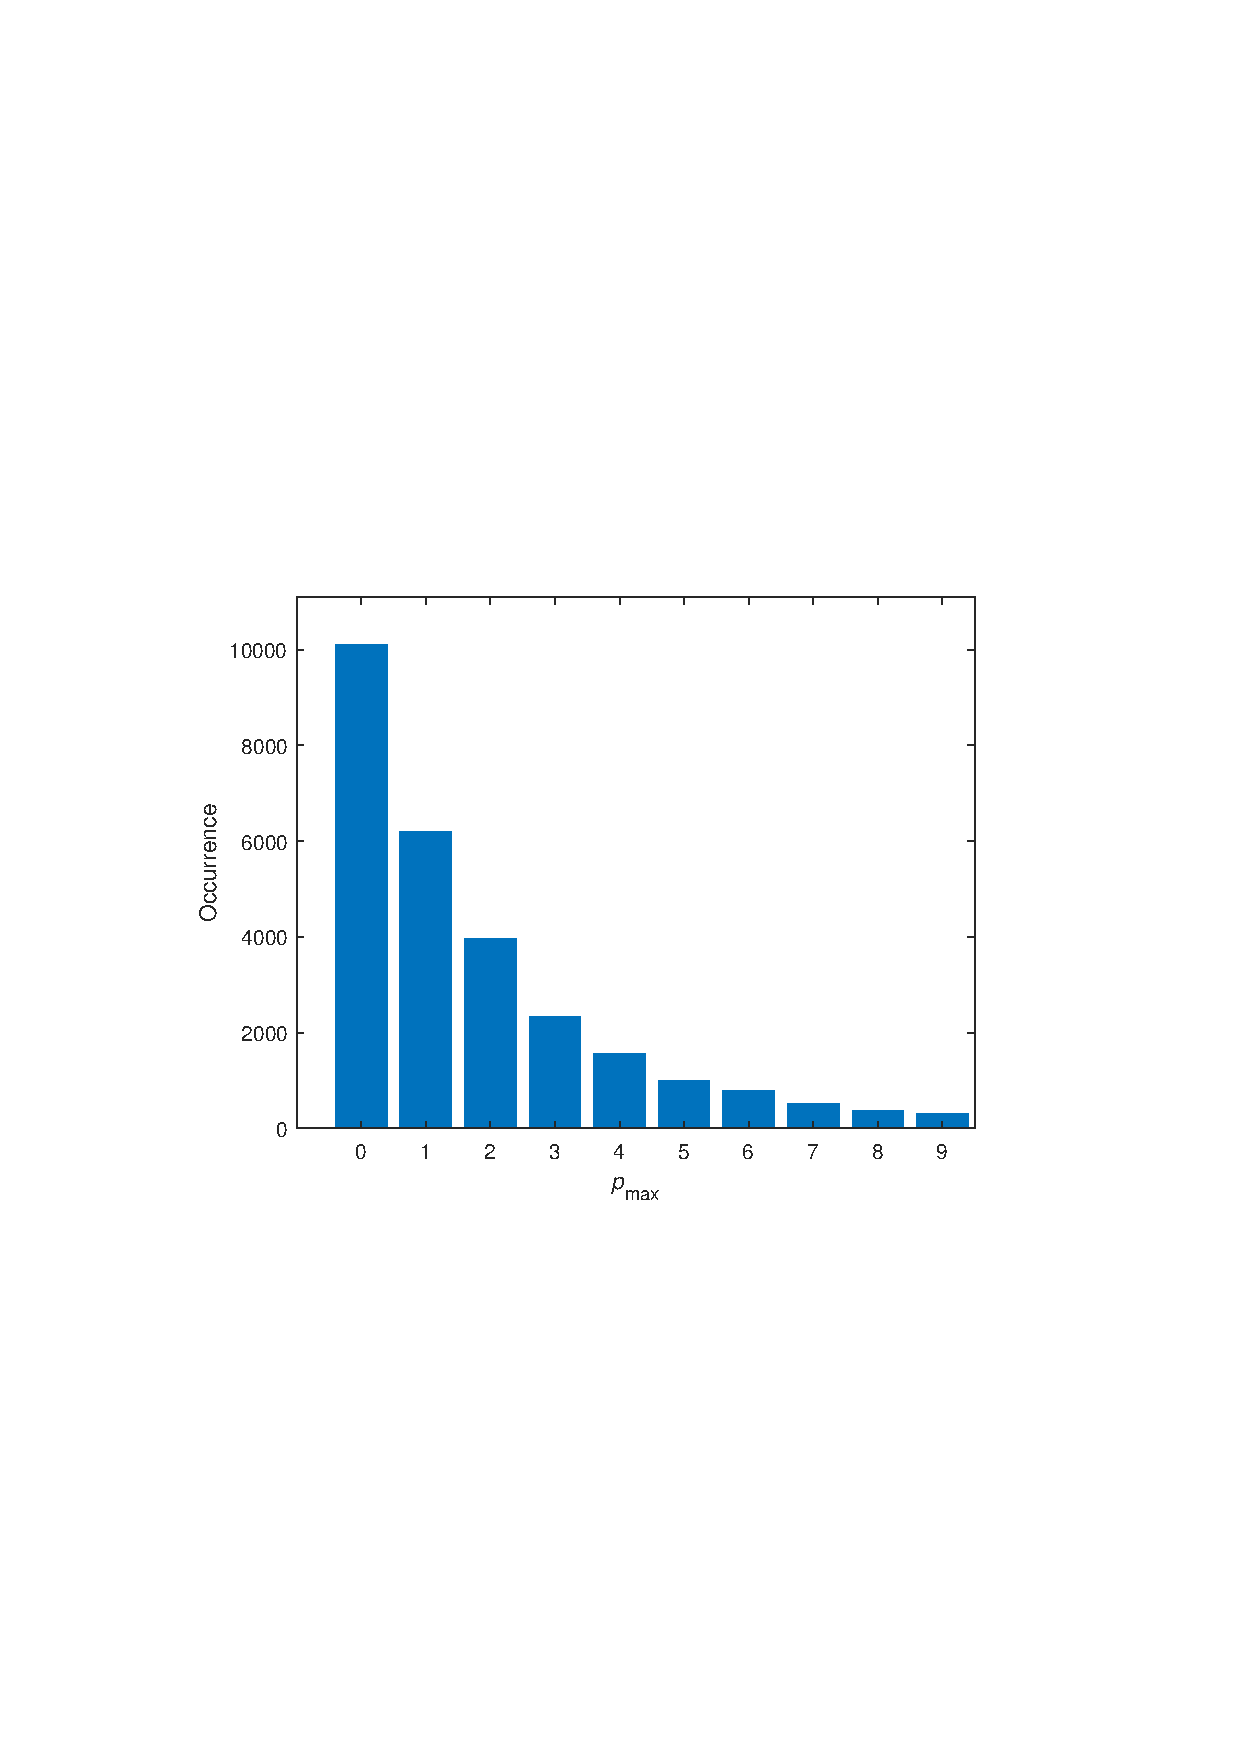
\includegraphics[width=0.35\textwidth]{figures/IPVO_Lena_3x3_hist.pdf}}
%    \caption{PEH of $p_{\rm max}$ by \eqref{eq:pmax} for the standard gray-scale $512 \times 512$ sized image Lena.}
%    \label{Fig.IPVO}
\centering
\subfigure[Original PVO-based method \cite{Li2013PVO}.]{
    \begin{minipage}[t]{0.32\linewidth}
    \centering
    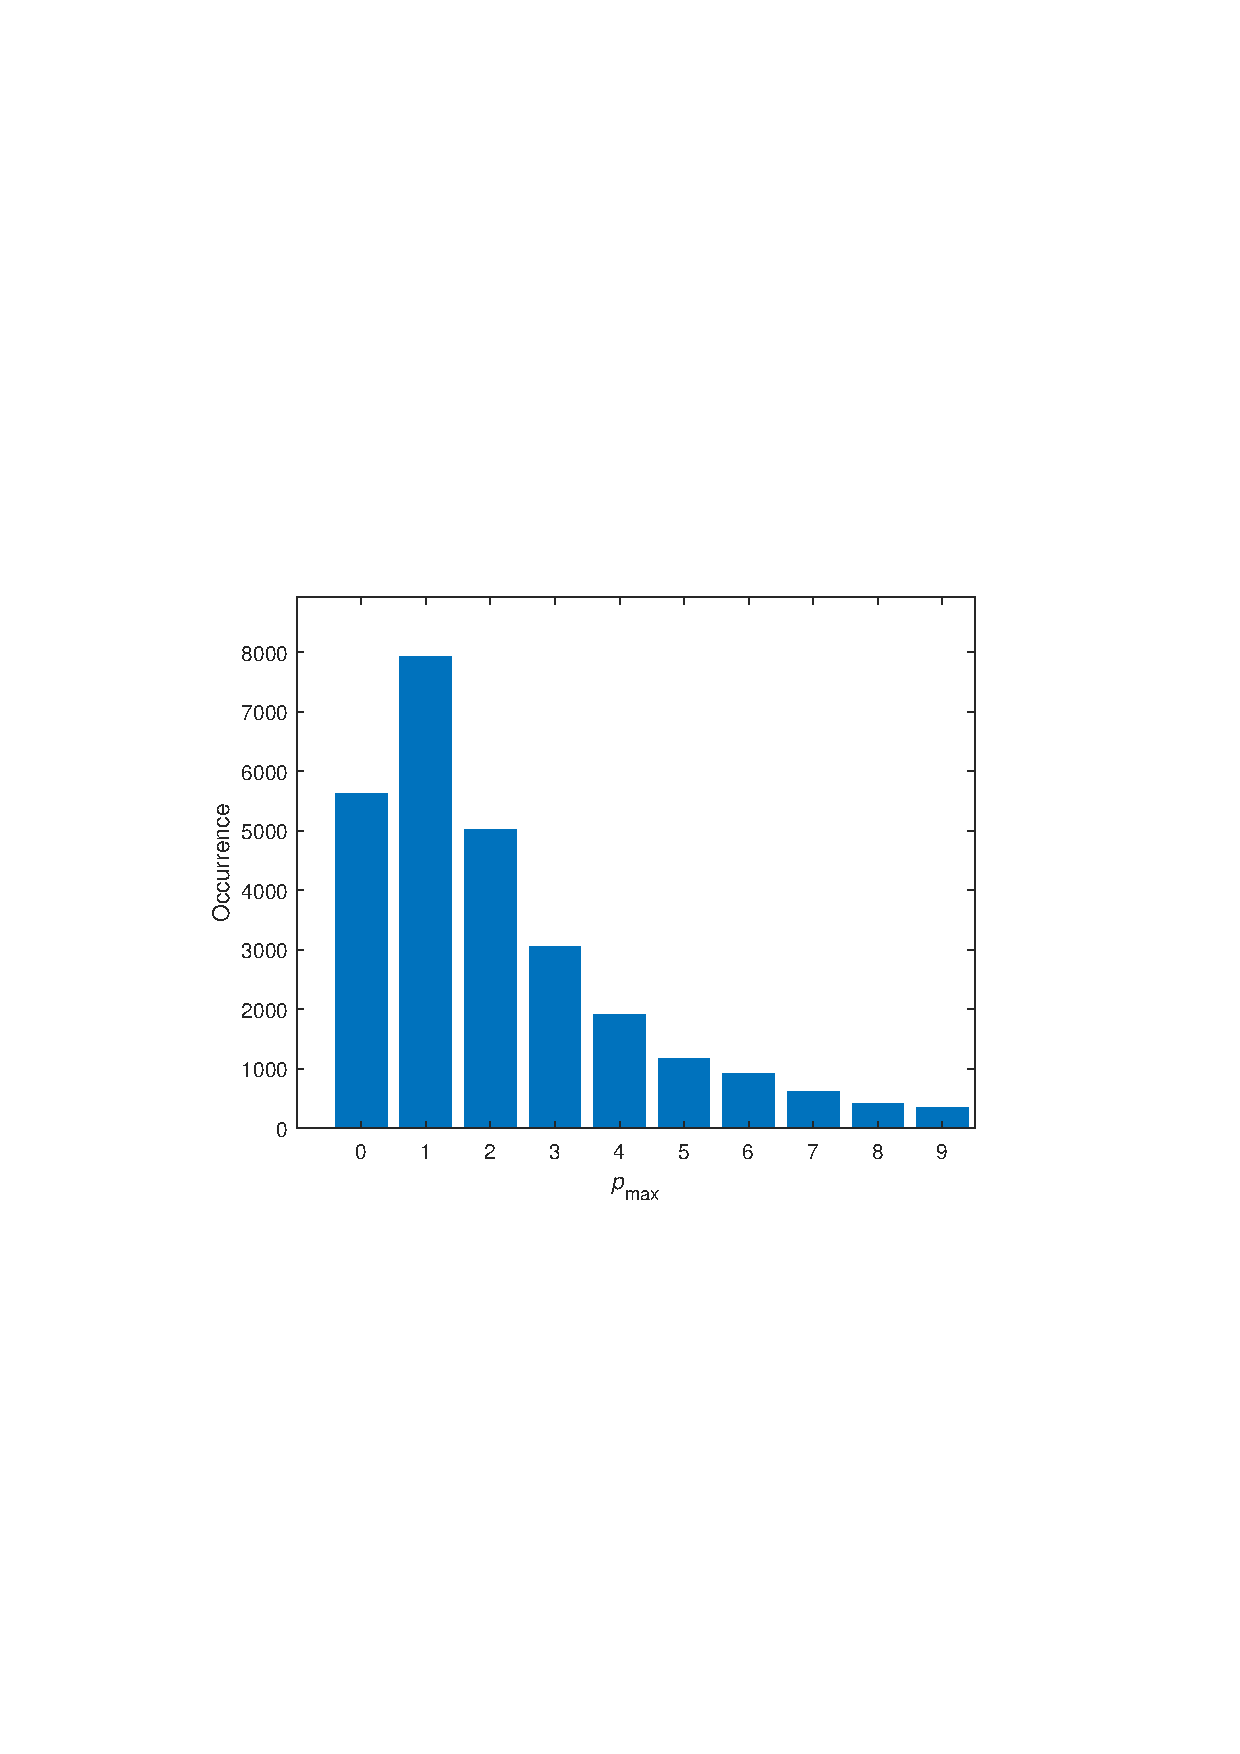
\includegraphics[width=1\textwidth]{figures/PVO_Lena_3x3_hist.pdf}
    \end{minipage}
}
\qquad
\subfigure[Improved PVO-based method \cite{Peng2014IPVO}.]{
    \begin{minipage}[t]{0.33\linewidth}
    \centering
    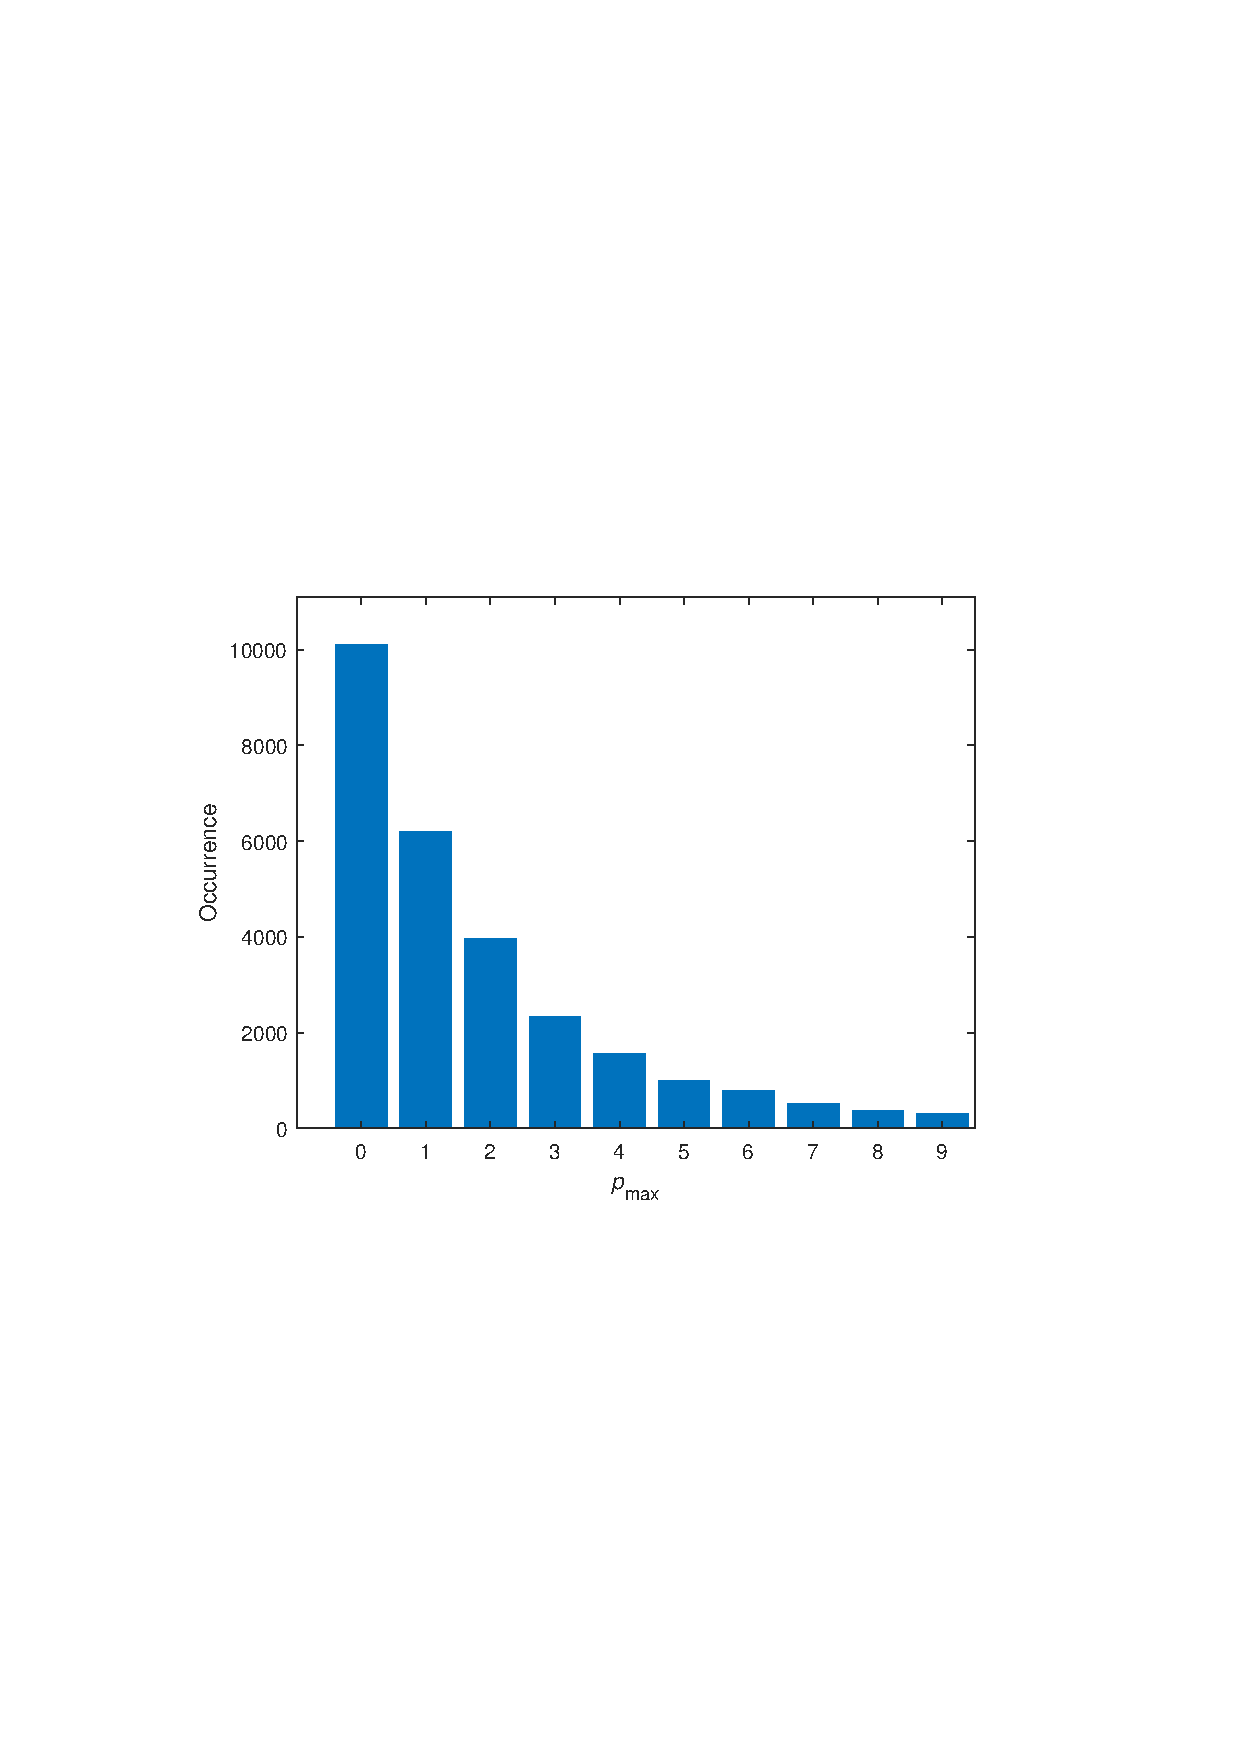
\includegraphics[width=1\textwidth]{figures/IPVO_Lena_3x3_hist.pdf}
    \end{minipage}
}		
\centering
\caption{PEH of $p_{\rm max}$ with block size $n = 3 \times 3$ for the standard gray-scale $512 \times 512$ sized image Lena.}
\label{Fig.PVOIPVO}
\end{figure*}

More clearly, prediction-error $p_{\rm max}$ is modified to derive the marked prediction-error $\hat{p}_{\rm max}$ by
\begin{equation}\label{eq:mpmax}
\hat{p}_{\rm max} = \left\{\begin{array}{ll}
p_{\rm max} + b, & \text{if } p_{\rm max}=0 \\
p_{\rm max} + 1, & \text{if } p_{\rm max}\geq 1 \\
\end{array}\right.,
\end{equation}
where $b \in \{0,1\}$ is one bit secret data to be embedded. And, the marked largest pixel $\hat{x}_{\xi(n)}$ is obtained by
\begin{equation}\label{eq:mpixel}
\hat{x}_{\xi(n)} = x_{\xi(n-1)} + \hat{p}_{\rm max}.
\end{equation}
In the improved PVO-based method, in each block, it is note that $\hat{x}_{\xi(n)} \geq x_{\xi(n)}$, and the PVO of the marked pixels $(\hat{x}_{\xi(1)},...,\hat{x}_{\xi(n)})$ is as the same as the original pixels, which guarantees the reversibility.

For the decoder, in each block, the marked prediction-error $\hat{p}_{\rm max}$ with pixels $(\hat{x}_{\xi(1)},...,\hat{x}_{\xi(n)})$ in ascending order is computed as
\begin{equation}\label{eq:dmpmax}
\hat{p}_{\rm max} = \left\{\begin{array}{ll}
\hat{x}_{\xi(n)} - \hat{x}_{\xi(n-1)},      & \text{if } \xi(n) > \xi(n-1) \\
\hat{x}_{\xi(n)} - \hat{x}_{\xi(n-1)} - 1,  & \text{if } \xi(n) < \xi(n-1)
\end{array}\right.,
\end{equation}
Next, the original pixel value $x_{\xi(n)}$ is recovered by
\begin{equation}\label{eq:dmpixel}
x_{\xi(n)} = \left\{\begin{array}{ll}
\hat{x}_{\xi(n)},       & \text{if } \hat{p}_{\rm max} = 0 \\
\hat{x}_{\xi(n)} - 1,   & \text{if } \hat{p}_{\rm max} \geq 1 \\
\end{array}\right.,
\end{equation}
while other marked pixels $(\hat{x}_{\xi(1)},...,\hat{x}_{\xi(n-1)})$ is recovered as themselves. And, the embedded secret data is 0 if $\hat{p}_{\rm max} = 0$ and 1 if $\hat{p}_{\rm max} = 1$.

Moreover, for each block, the similar process is applied to the smallest pixel value $x_{\xi(1)}$ by computing the prediction-error $p_{\rm min}$ as
\begin{equation}\label{eq:pmin}
p_{\rm min} = \left\{\begin{array}{ll}
x_{\xi(2)} - x_{\xi(1)},      & \text{if } \xi(2) > \xi(1) \\
x_{\xi(2)} - x_{\xi(1)} - 1,  & \text{if } \xi(2) < \xi(1)
\end{array}\right.,
\end{equation}
where pixel $p_{\rm min} \geq 0$. And the PEH of $p_{\rm min}$ peaks at 0 as well. The detail embedding and extraction process is described in \cite{Peng2014IPVO}.


\subsection{Pixel-based PVO RDH \cite{Qu2015PPVO}}\label{sec:2.2}
In the classical PVO-based RDH method such as the original PVO-base method \cite{Li2013PVO} and the improved PVO-based method \cite{Peng2014IPVO}, the cover image is first devided into equal size and non-overlapping blocks. The sorted pixels $(x_{\xi(2)},...,x_{\xi(n-1)})$ is not utilized in the embedding process and the total number of prediction-errors is bounded by the block constraint, which causing the difficulty of efficient embedding data into smooth region. In \cite{Qu2015PPVO}, Qu \emph{et al.} propose a pixel-based PVO RDH method, which is called PPVO, to utilized the sorted pixels for data embedding.

PPVO achieves an pixel-by-pixel data embedding process. For current pixel, the context pixels defined as the pixels in the lower right direction and form an vector $C=\{c_1,...,c_{\rm CN}\}$ shown in Fig. \ref{Fig.PPVOCNandHist}(a), where the number of context pixels is defined as ${\rm CN}$.
\begin{figure*}
\centering
\subfigure[Context pixels of $x$.]{
    \begin{minipage}[t]{0.22\linewidth}
    \centering
    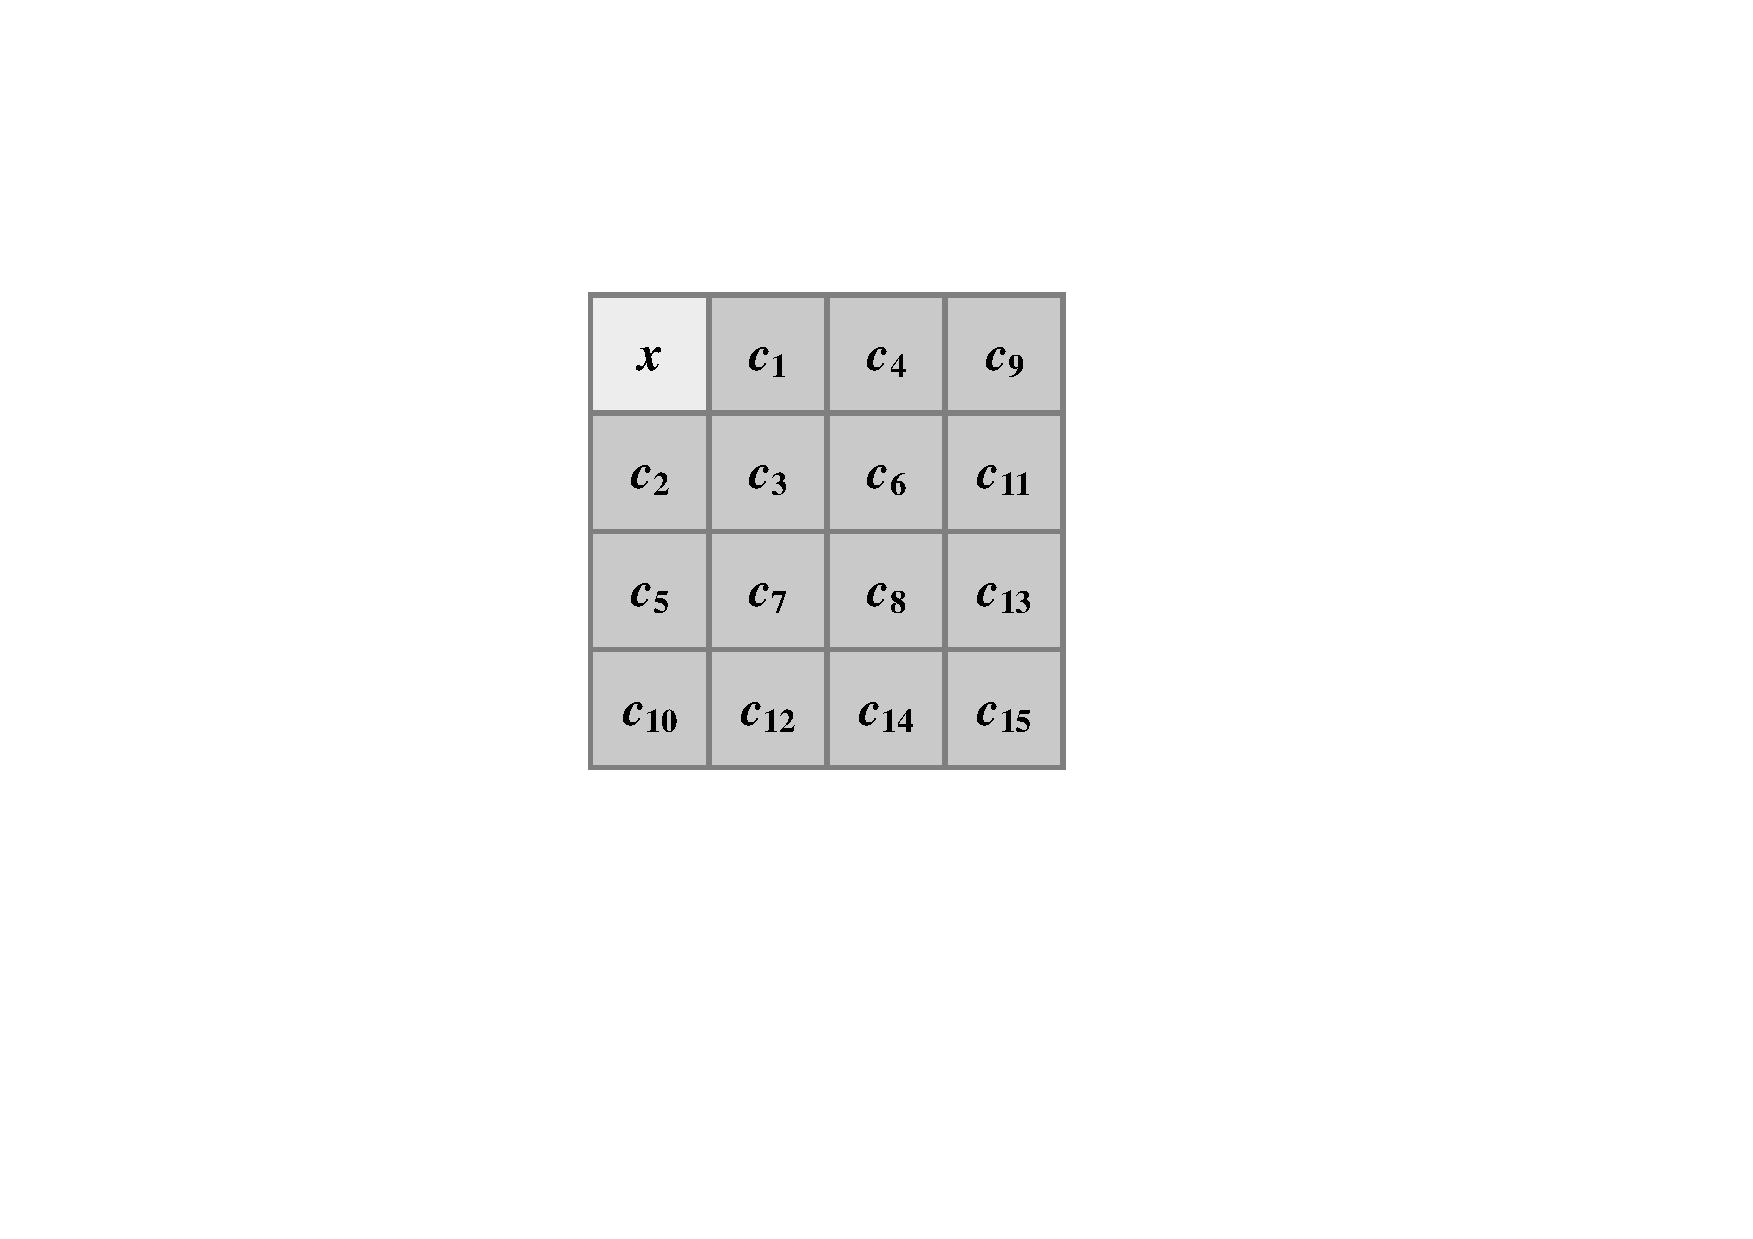
\includegraphics[width=1\textwidth]{figures/PPVOContext.pdf}
    \end{minipage}
}
\qquad\qquad
\subfigure[PEH of $p$ by \eqref{eq:PPVOPE}.]{
    \begin{minipage}[t]{0.31\linewidth}
    \centering
    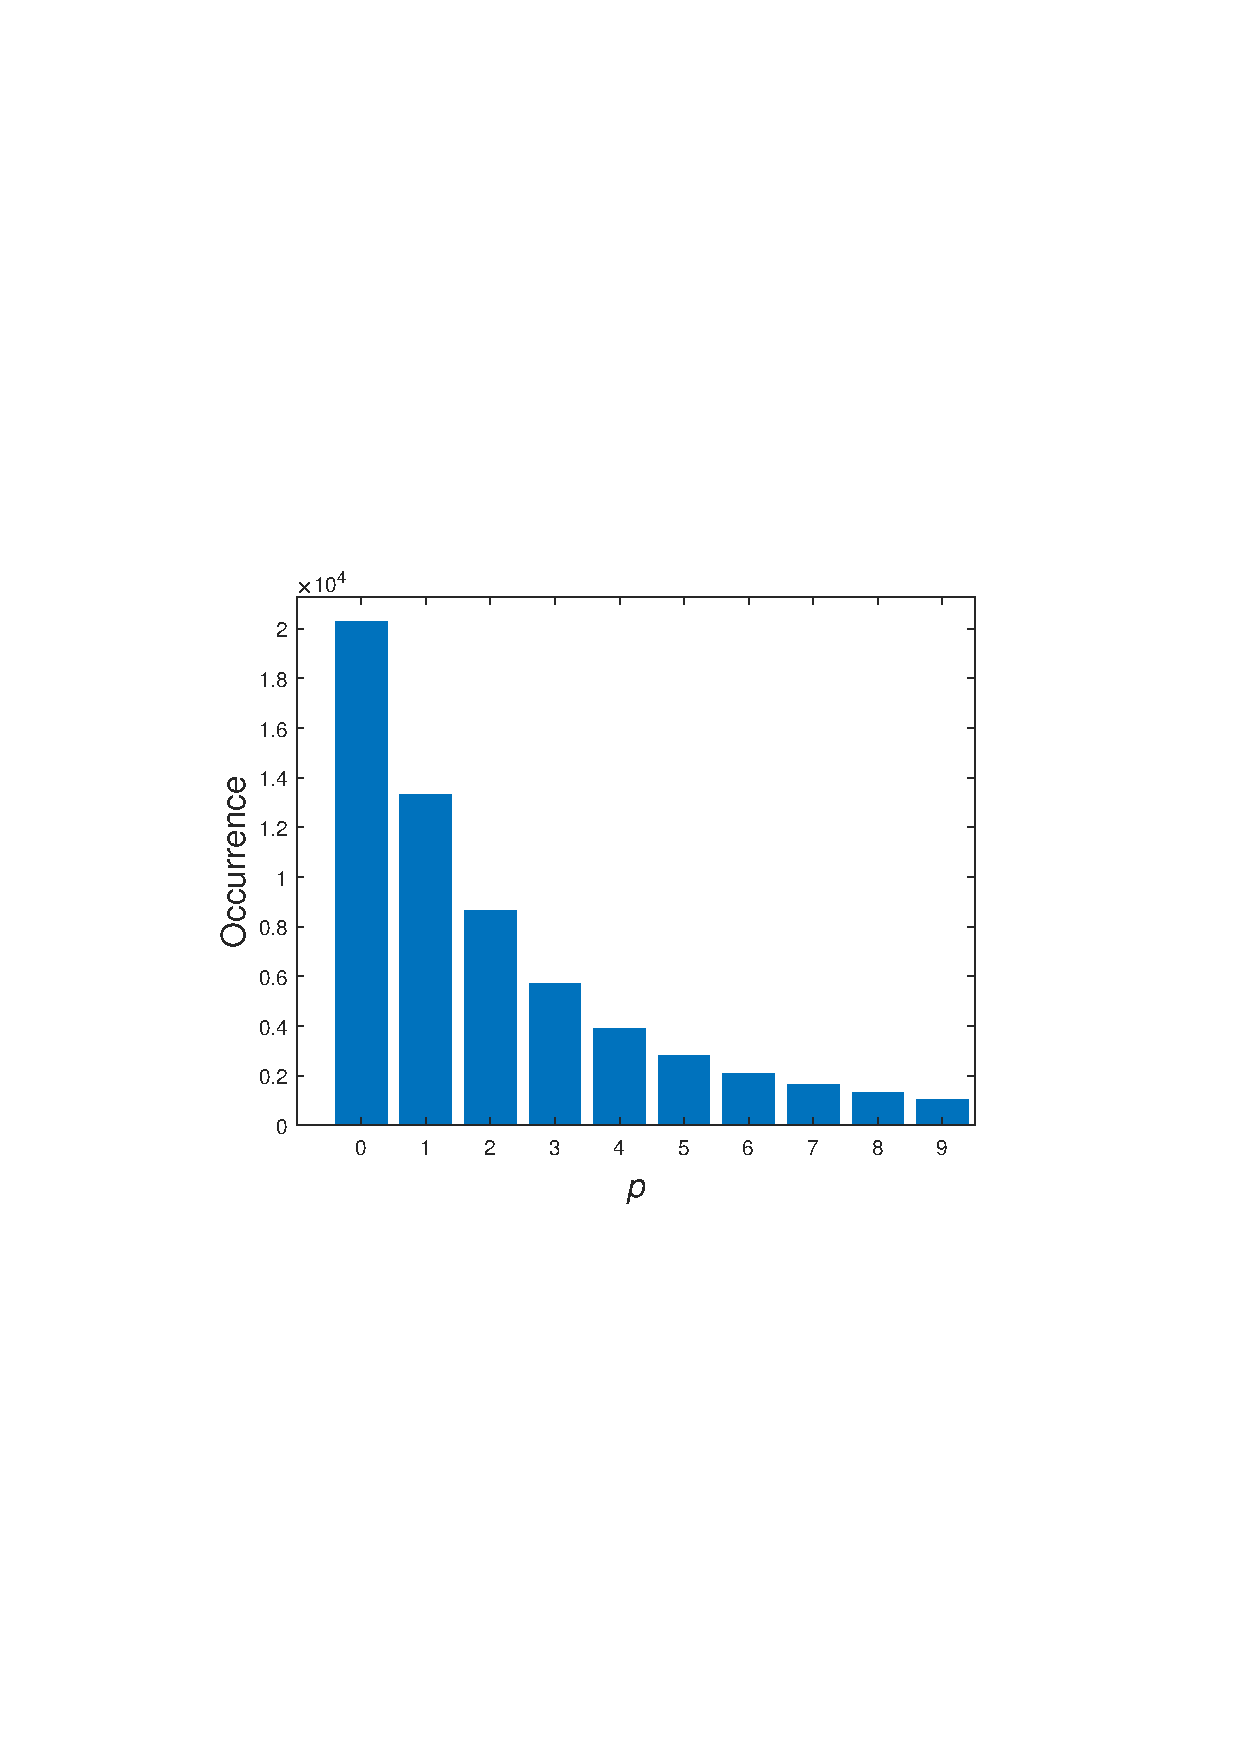
\includegraphics[width=1\textwidth]{figures/PPVO_Lena_CN15_hist.pdf}
    \end{minipage}
}		
\centering
\caption{PPVO Context Pixels and show the shaper histogram with $CN = 15$.}
\label{Fig.PPVOCNandHist}
\end{figure*}

Before describe the prediction algorithm, to simplify the explanation, pixels participating in the embedding process are grouped into four sets, which are
\begin{equation*}\label{eq:PPVOCNandHist}
\begin{array}{ll}
S_1 = \{ x | \max(C) \neq \min(C), x \geq \max(C) \} \\
S_2 = \{ x | \max(C) \neq \min(C), x \leq \min(C) \} \\
S_3 = \{ x | \max(C)   =  \min(C), x \leq \min(C), \min(C) \neq 254 \} \\
S_4 = \{ x | \max(C)   =  \min(C), x \geq \min(C), \min(C)   =  254 \} \\
\end{array}.
\end{equation*}
Then, for each pixel $x$, the prediction-error $p$ is calculated by
\begin{equation}\label{eq:PPVOPE}
p = \left\{\begin{array}{ll}
x - \max(C),    & \text{if } x \in S_1  \\
\min(C) - x,    & \text{if } x \in S_2 \cup S_3 \\
0,              & \text{if } x \in S_4 \\
{\rm skip},     & \text{otherwise}
\end{array}\right.,
\end{equation}
where prediction-error $p$ is located in the interval of $[0, \infty)$. More specifically, PEH of $p$ peak at 0 as shown in Fig. \ref{Fig.PPVOCNandHist}(b) so that $p$ is modified to derive the marked prediction-error $\hat{p}$ by
\begin{equation}\label{eq:PPVOMPE}
\hat{p} = \left\{\begin{array}{ll}
p + b,  & \text{if } p = 0      \\
p + 1,  & \text{if } p \geq 1
\end{array}\right.,
\end{equation}
where $b \in \{0,1\}$ is one bit secret data to be embedded. And the marked pixel $\hat{x}$ is obtained by
\begin{equation}\label{eq:PPVOMPixel}
\hat{x} = \left\{\begin{array}{ll}
\max(C) + \hat{p},  & \text{if } x \in S_1 \\
\min(C) - \hat{p},  & \text{if } x \in S_2 \cup S_3 \\
\min(C) + \hat{p},  & \text{if } x \in S_4 \\
{\rm skip},         & \text{otherwise}
\end{array}\right..
\end{equation}

In this method, for each pixel satisfying $x \notin S_4$, marked pixel satisfies $\hat{x} \geq x$ if $x \geq \max(C)$ and $\hat{x} \leq x$ if $x \leq \min(C)$ which ensures reversibility.
And reason of processing the pixels $x \in S_4$ specially is that pixels equal 255 are modified to 254 during the location map stage and $x \in S_4$ is increased by 1 or 0 can decrease the distortion of data embedding. It is note that, in the embedding process, the proper $NC$ is selected by choosing the best result of $C = \{1,...,i\}(i \in {1,...,15})$ exhaustively.

For the decoder, to extract data and recover the ordinal pixel, the same marked prediction-error $\hat{p}$ of current pixel $x$ is calculated by
\begin{equation}\label{eq:PPVOdMinNeqMax}
\hat{p} = \left\{\begin{array}{ll}
\hat{x} - \max(C),  & \text{if } \hat{x} \in S_1  \\
\min(C) - \hat{x},  & \text{if } \hat{x} \in S_2 \cup S_3 \\
\hat{x} - \min(C),  & \text{if } \hat{x} \in S_4  \\
{\rm skip},         & \text{otherwise}
\end{array}\right..
\end{equation}
In addition, the original pixel value $x$ is recovered by
\begin{equation}\label{eq:PPVOdMPixel}
x = \left\{\begin{array}{ll}
\hat{x},        & \text{if } \hat{p} = 0 \\
\hat{x} - 1,    & \text{if } \hat{x} \in S_1 \cup S_4 \text{ and } \hat{p} \geq 1 \\
\hat{x} + 1,    & \text{if } \hat{x} \in S_2 \cup S_3 \text{ and } \hat{p} \geq 1 \\
{\rm skip},         & \text{otherwise}
\end{array}\right..
\end{equation}
With the recover process, the secret data is extracted that $b = 1$ if $\hat{p}=1$ and $b = 0$ if $\hat{p} = 0$.

The experimental results show that PPVO gets a large maximum embedding capacity than the previous PVO-based method \cite{Li2013PVO,Peng2014IPVO} by pixel-by-pixel embedding. And it obtains a sharper histogram which is causing a result of better performance as shown in Fig. \ref{Fig.PPVOCNandHist}.

%----------------------------------------------------------------------------------------
\section{Proposed Method}\label{sec:3}
% motivation and simply description
In this section, a extended PPVO predictor is first introduced. Then, a multi-size based embedding method for MHM is proposed to further improve the performance. Finally, the embedding procedure and extraction procedure is described.

\subsection{Extended PPVO predictor}\label{sec:3.1}
Compared with PVO-based methods such as PVO\cite{Li2013PVO}, IPVO\cite{Peng2014IPVO} and PVO-\emph{k}\cite{Ou2014PVOk}, in PPVO, every pixel is predicted by context pixels, breaking through the block constraint. In PPVO, to ensure reversibility, pixels in lower right direction are utilized as context region to predict the current pixel which is shown in Fig. \ref{Fig.Context}(a). The prediction is more accurate, however, the surrounding context information is not fully utilized. There are some other pixels are omitted which is beneficial to provide more useful information for prediction. Clearly, for example, in Fig. \ref{Fig.Context}(b), pixels $\{c_{4}, c_{9}, c_{10}, c_{12}, c_{17}, c_{18}, c_{21}, c_{22}, c_{24}\}$ in left lower direction should be used in prediction procedure as one part of context pixels which is omitted in PPVO. Then the extended PPVO predictor is introduced to show how to make better prediction.
\begin{figure*}
\centering
\subfigure[PPVO.]{
    \begin{minipage}[t]{0.21\linewidth}
    \centering
    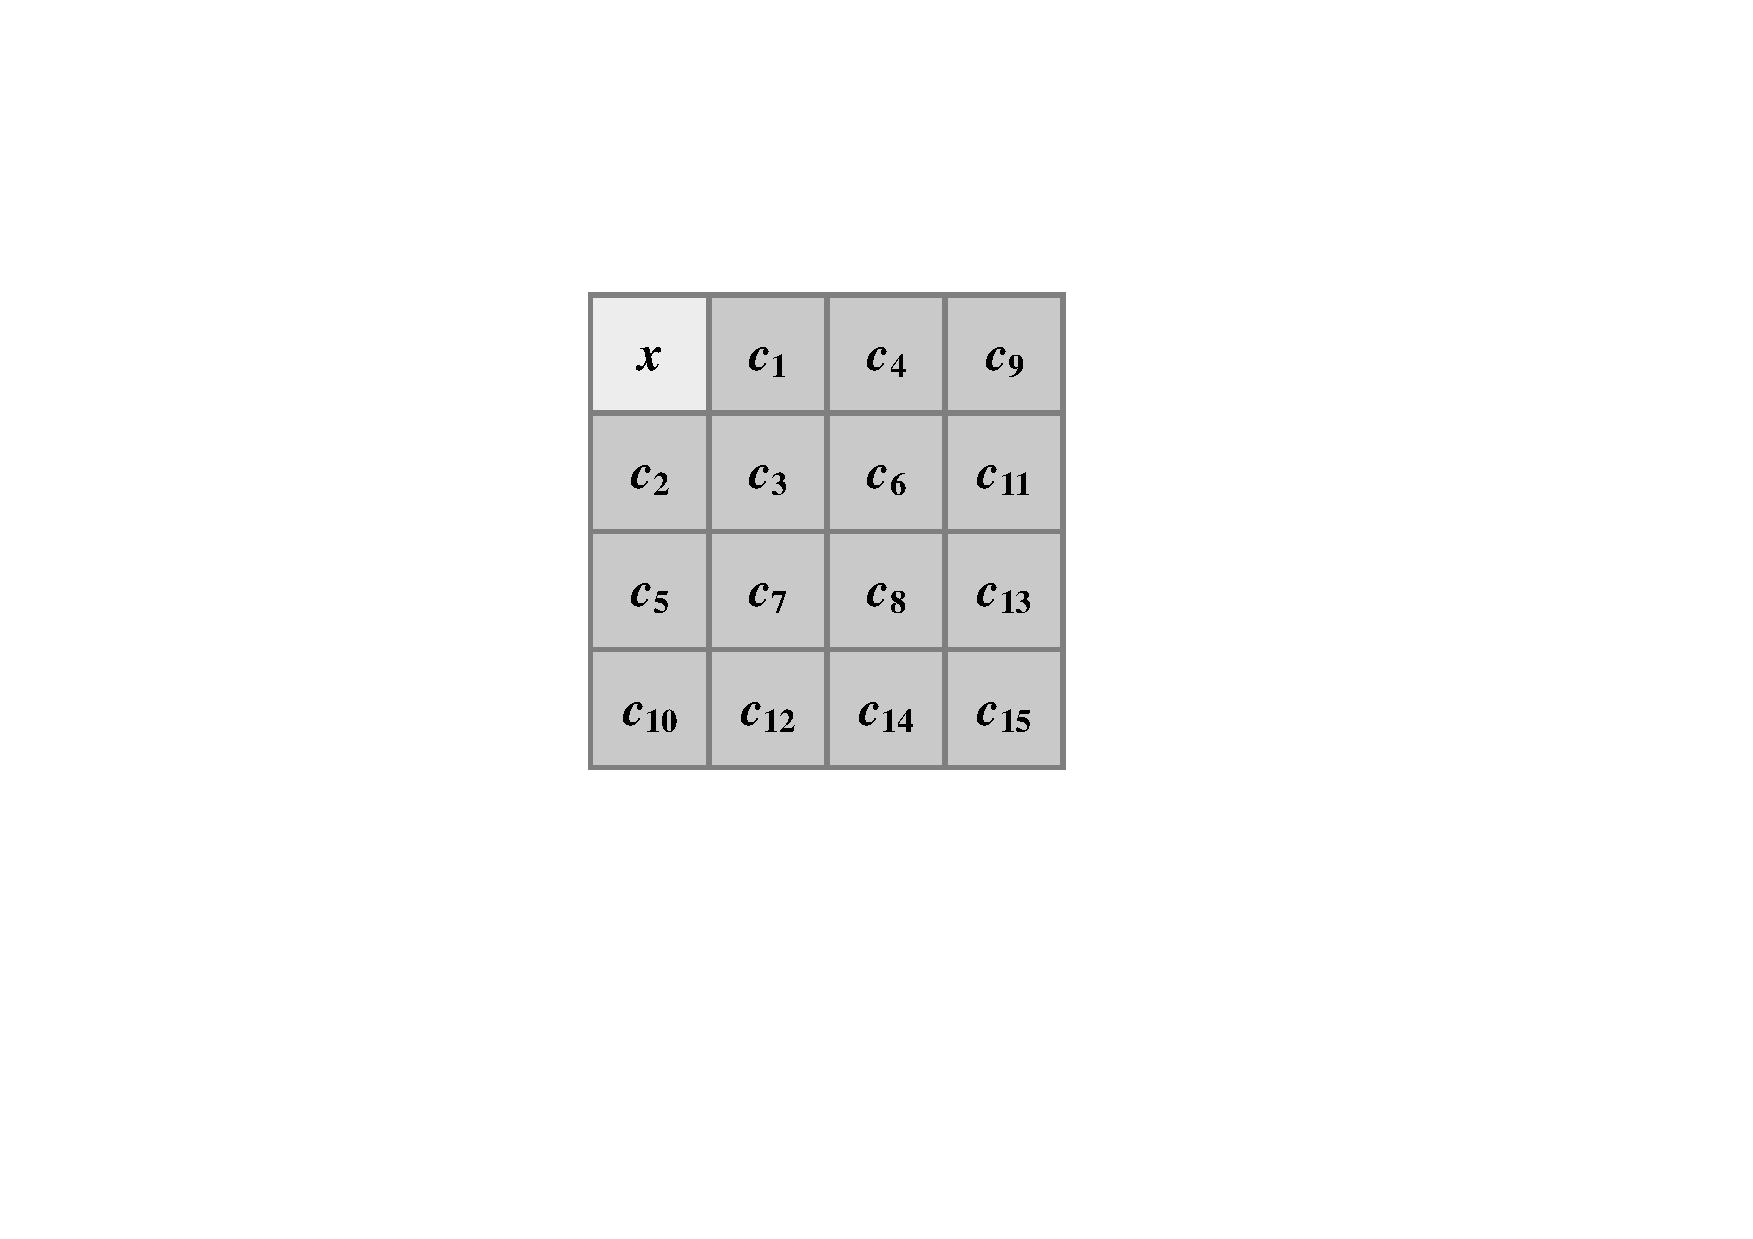
\includegraphics[width=1\textwidth]{figures/PPVOContext.pdf}
    \end{minipage}
}
\qquad\qquad
\subfigure[Extended PPVO.]{
    \begin{minipage}[t]{0.37\linewidth}
    \centering
    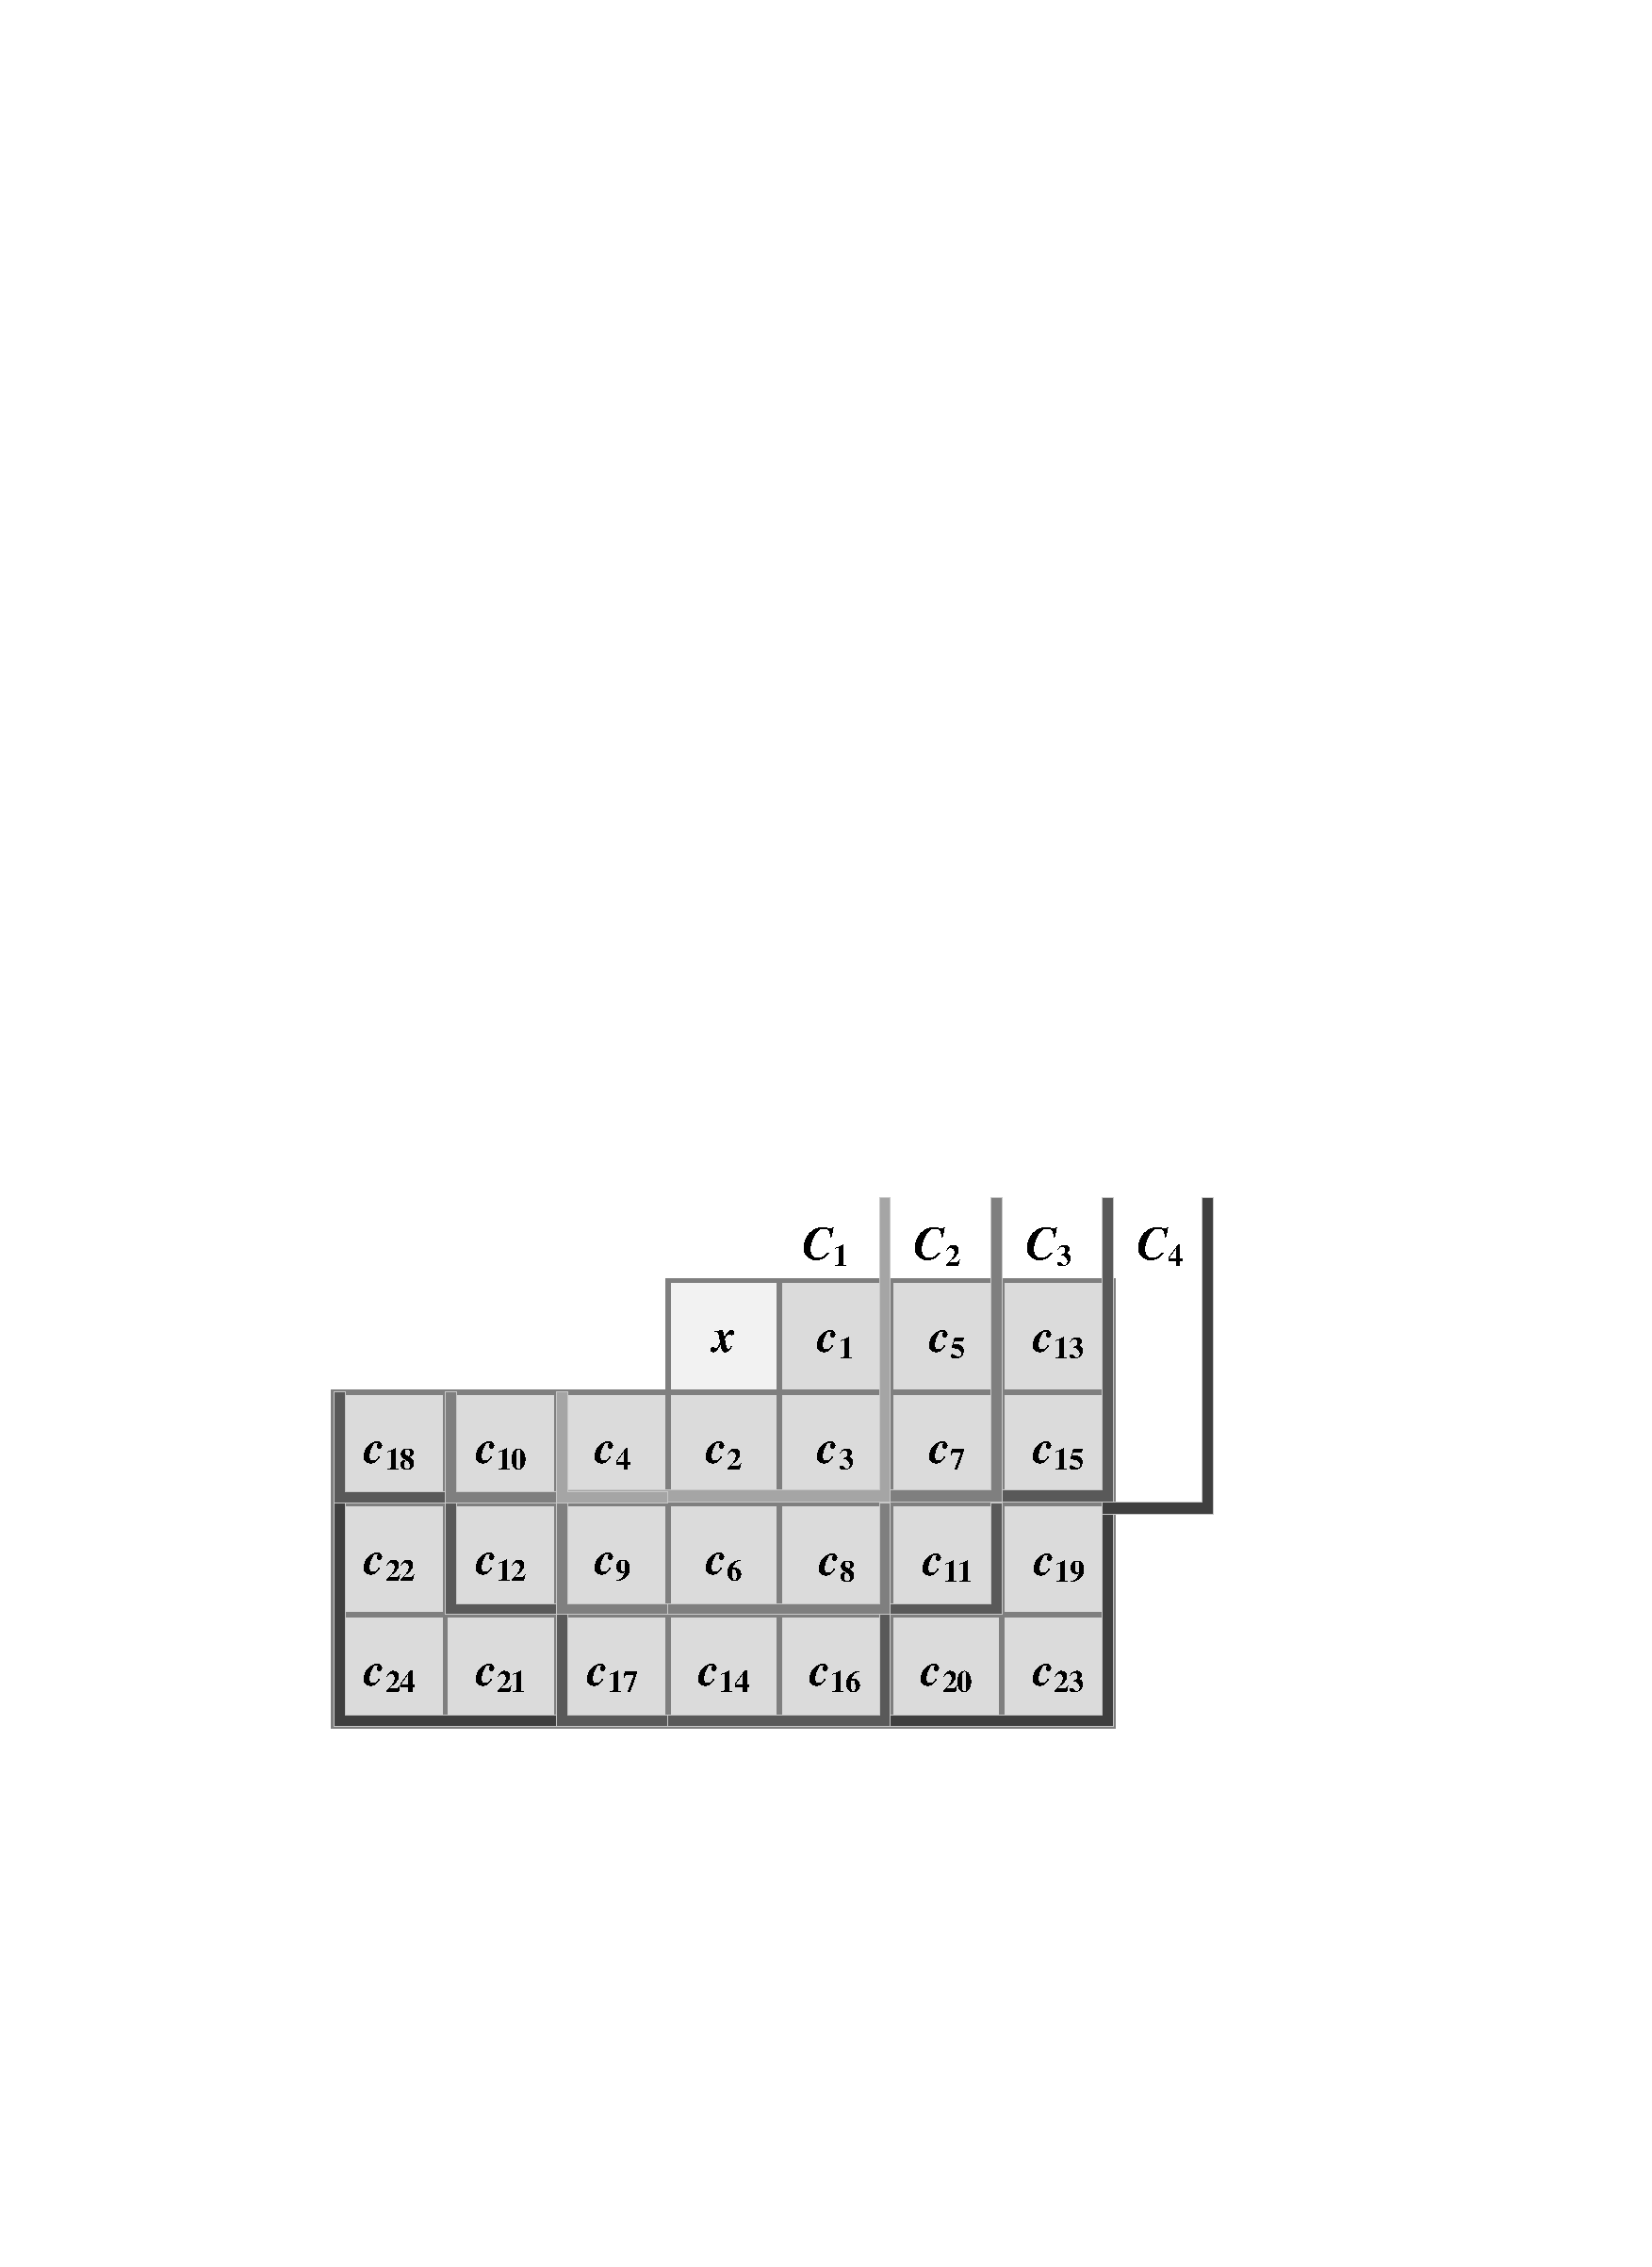
\includegraphics[width=1\textwidth]{figures/ExtendedPPVOContext.pdf}
    \end{minipage}
}		
\centering
\caption{Context pixels of PPVO(left) and Extended PPVO(right).}
\label{Fig.Context}
\end{figure*}

Here, the symbol definitions are the same as the definitions in section \ref{sec:2}. In Fig. \ref{Fig.Context}, the number of context pixels is $CN = 24$, where context pixel vector is $C = (c_{1}, ..., c_{24})$. And the prediction procedure is described as follow. Compared with PPVO, except the four sets $S_1, S_2, S_3$ amd $S_4$, another set is defined as
\begin{equation*}\label{eq:PPVOCNandHist}
\begin{array}{ll}
S_5 = \{ x | \max(C)   =  \min(C), x > \max(C), \max(C)   \neq  254 \} \\
\end{array}.
\end{equation*}
And, for each pixel $x$, the prediction-error is calculated by
\begin{equation}\label{eq:EPPVOPE}
p = \left\{\begin{array}{ll}
x - \max(C),    & \text{if } x \in S_1  \\
\min(C) - x,    & \text{if } x \in S_2 \cup S_3 \\
0,              & \text{if } x \in S_4 \\
x - \max(C) - 1,& \text{if } x \in S_5  \\
{\rm skip},     & \text{otherwise}
\end{array}\right.,
\end{equation}
where prediction-error $p$ is located in the interval of $[0, \infty)$. By the extended PPVO predictor, with the situation of $\max(C) = \min(C)$, pixel $x$ satisfying $x > \max(C)$ is utilized to obtain prediction-errors. More pixels participate in prediction procedure, leading to an increase in embedding capacity.

% show the example of histogram, comparatione and reasons.
% NL = max(C)-min(C)
For extended PPVO predictor, more surrounding pixels are fully considered as pixel context to predict current pixel, aiming to get sharper histogram. To show the superiority of extended PPVO predictor, compared with Qu \emph{et al.}' method, an comparison shown in Fig. \ref{Fig.ComparisonEPPVO}. In the example, eight standard gray-scale $512 \times 512$ sized images  are used and comparison of normalized PEHs of proposed extended PPVO predictor and PPVO predictor are displayed on the same figures. 
For extended PPVO predictor, pixels $\{c_{1}, c_{2}, c_{3}, c_{4}, c_{5}, c_{6}, c_{9}, c_{10}\}$ in Fig. \ref{Fig.Context}(b) are seen as context pixels, and for PPVO predictor, pixels $\{c_{1}, ..., c_{8}\}$ in Fig. \ref{Fig.Context}(a) are seen as context pixels. It is obviously that normalized PEHs of extended PPVO predictor have higher peaks at $0$, and the distributions are sharper, which is beneficial to the final embedding performance. Moreover, in the next data embedding procedure, pixels of $p = 0$ are used to embed secret data by expanding and others are shifted to ensure reversibility. Thus, we use embedding distortion of one bit data embedding to evaluate the distortion caused by histograms theoretically, numerically expressed as
\begin{equation*}\label{eq:EvaluateHistogram}
{\rm \mathbf{Eval}} = \frac{{\rm H}(0)}{\frac{1}{2}{\rm H}(0)+ \sum_{i \geq 1}{\rm H}(i)},
\end{equation*}
where ${\rm H}$ is the PEH and ${\rm H}(i)$ is the frequency of pixels whose prediction-errors $p = i$. This evaluation describes the distortion caused by embedding one bit data on ${\rm H}$. In Lena, Baboon and Airplane, ${\rm \mathbf{Eval}}$ of extended PPVO predictor are 2.07, 6.88 and 1.44 respectively, while value of evaluation are 2.81, 7.90 and 1.76 of PPVO predictor. It shows that data embedding on PEH of extended PPVO predictor may carry less distortion so that better performance can be obtained.
\begin{figure*}
\centering
\subfigure[Lena]{
    \begin{minipage}[t]{0.225\linewidth}
    \centering
    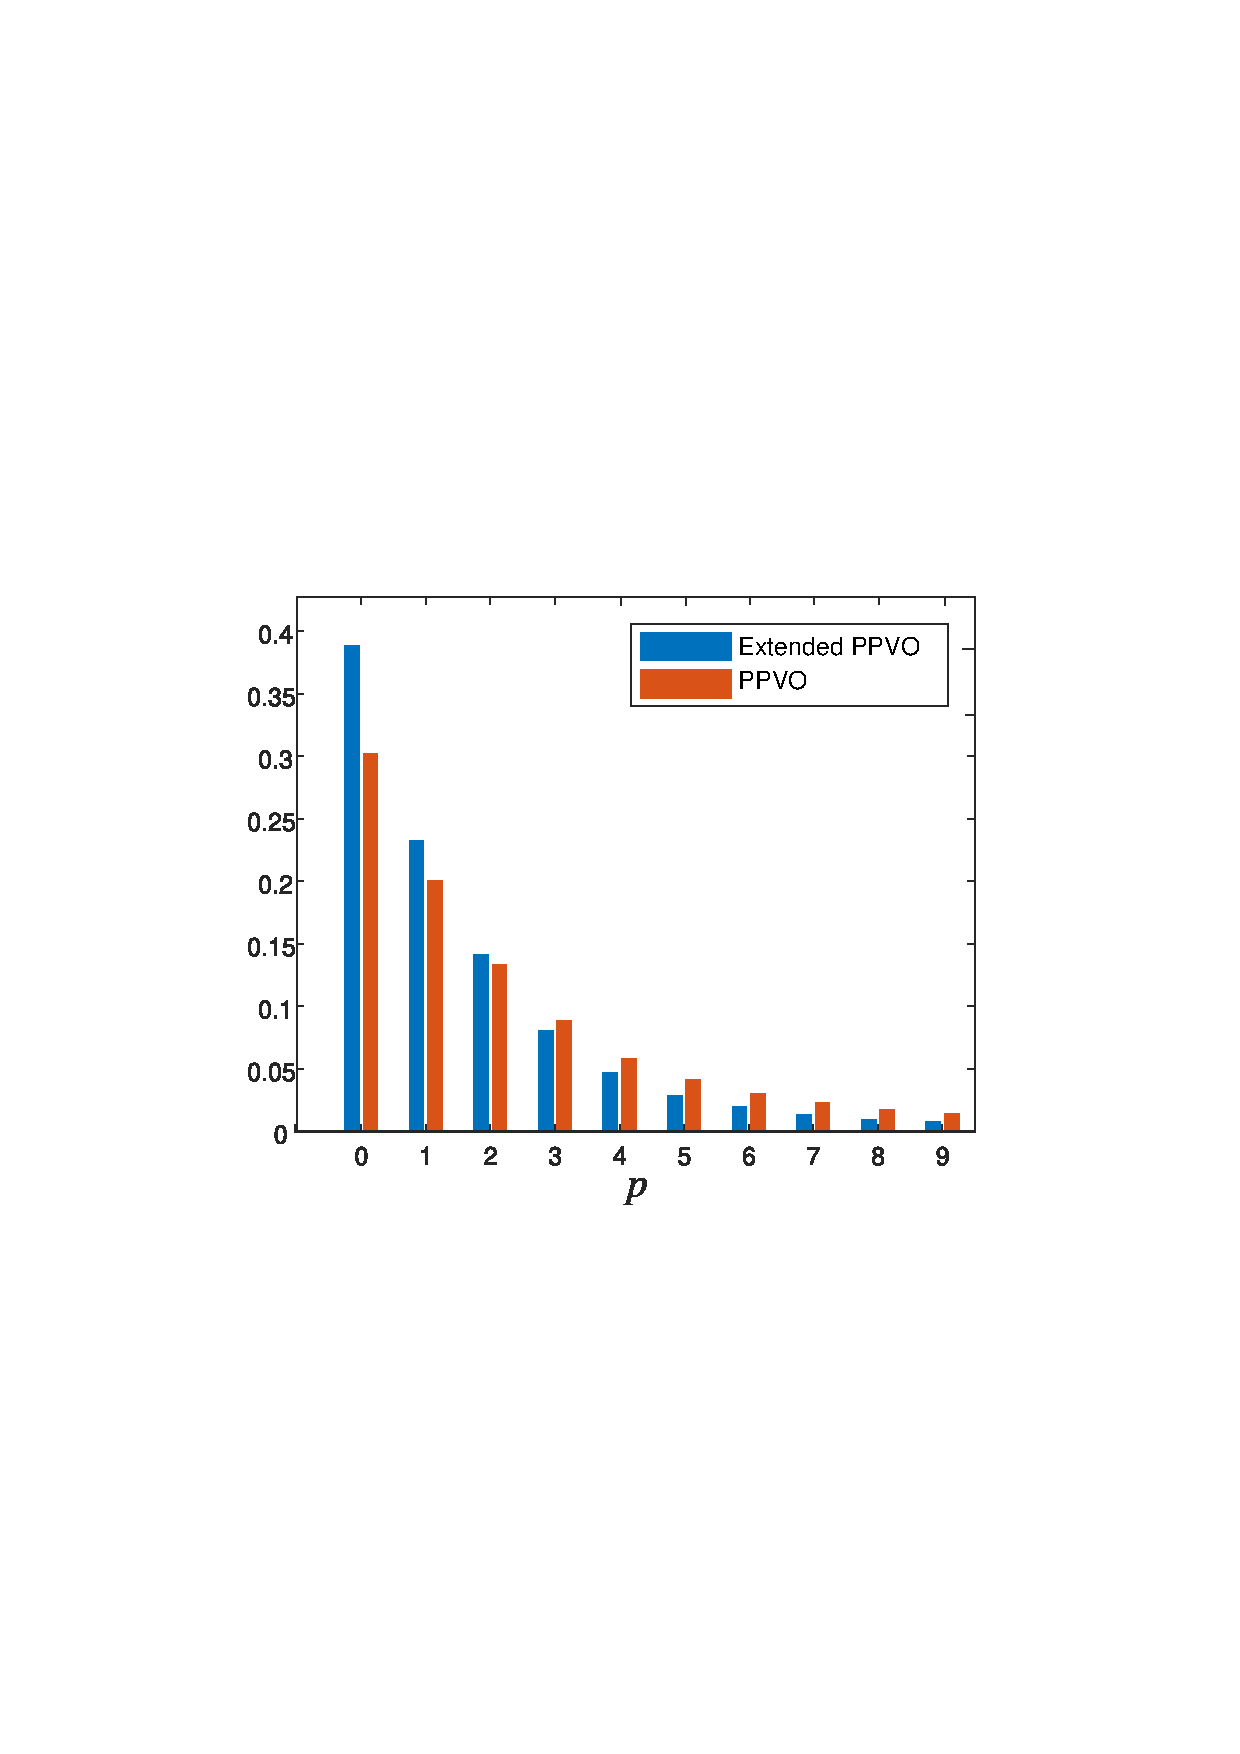
\includegraphics[width=1\textwidth]{figures/Comparison/lena.pdf}
    \end{minipage}
}
\subfigure[Baboon]{
    \begin{minipage}[t]{0.225\linewidth}
    \centering
    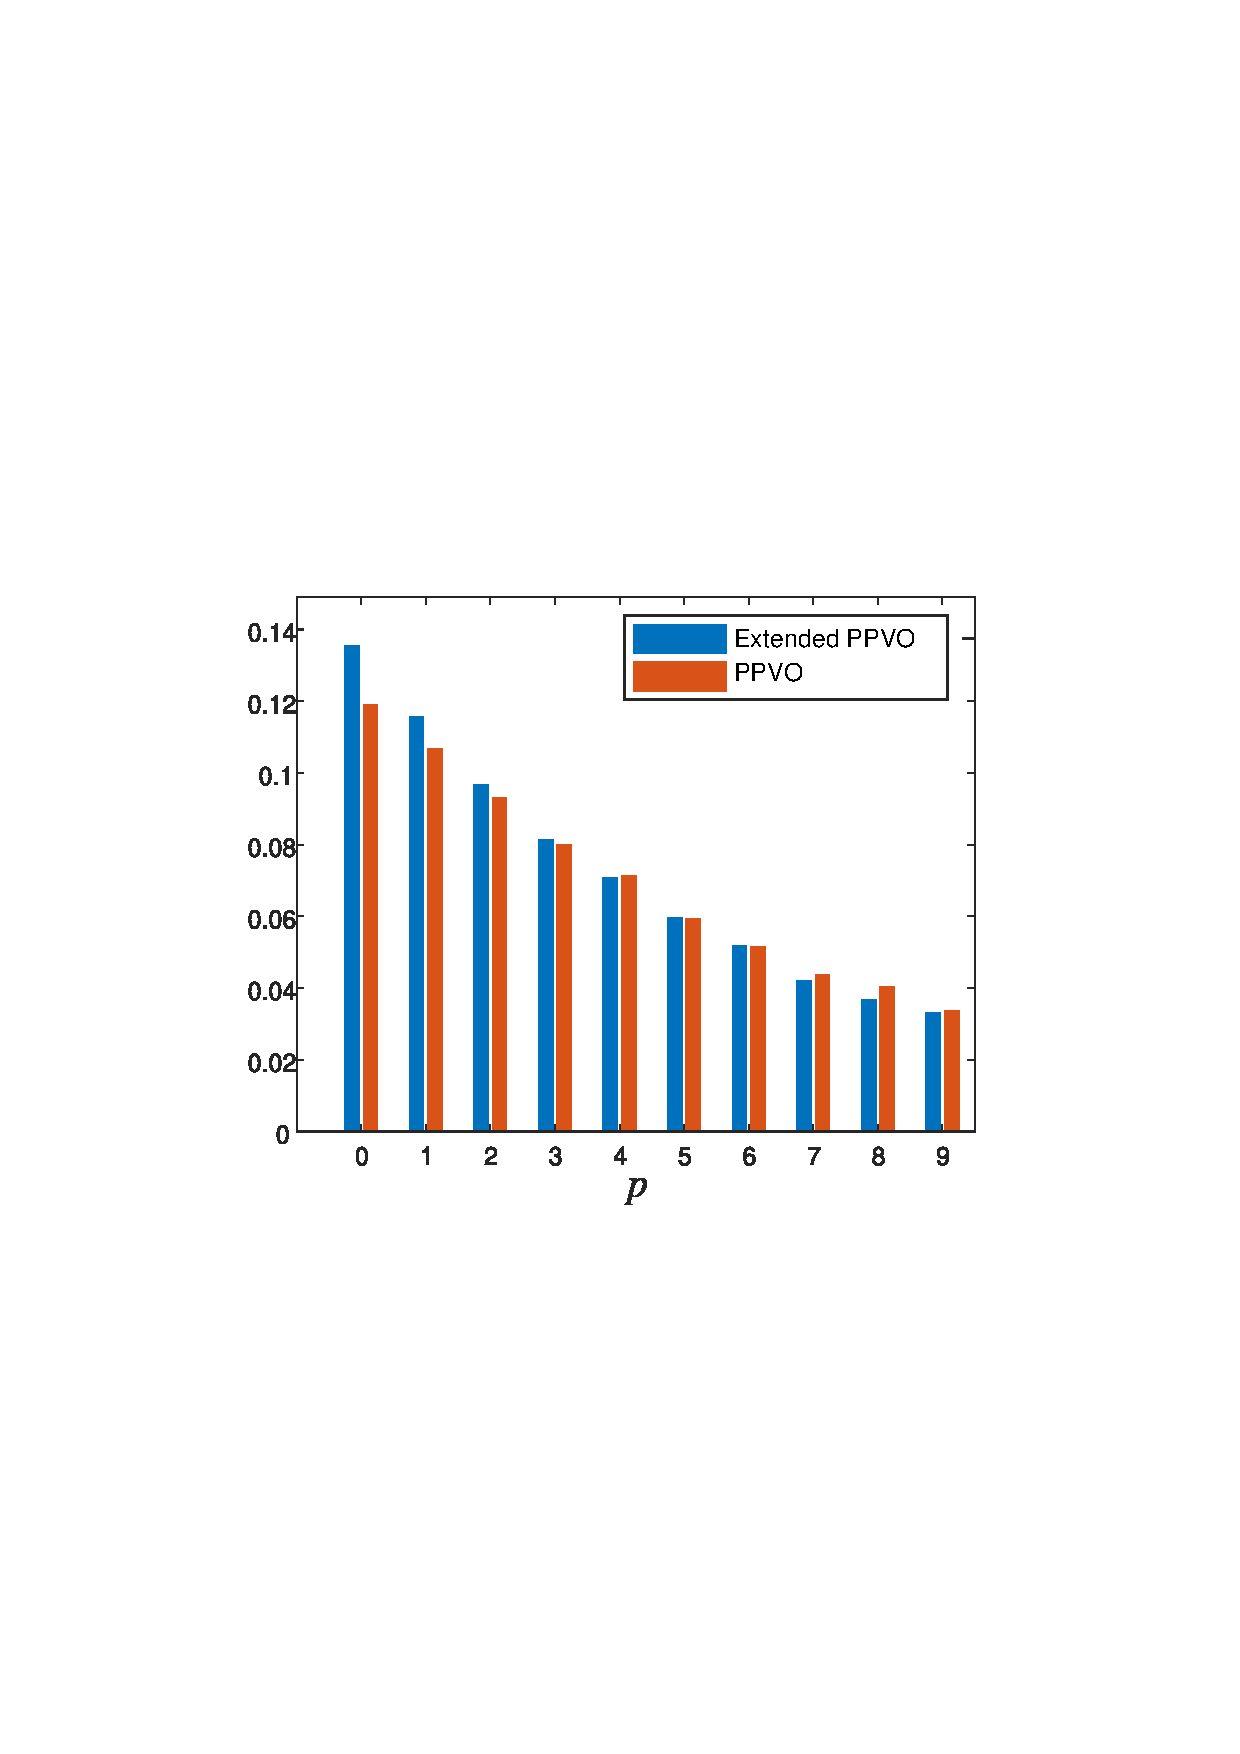
\includegraphics[width=1\textwidth]{figures/Comparison/baboon.pdf}
    \end{minipage}
}
\subfigure[Airplane]{
    \begin{minipage}[t]{0.225\linewidth}
    \centering
    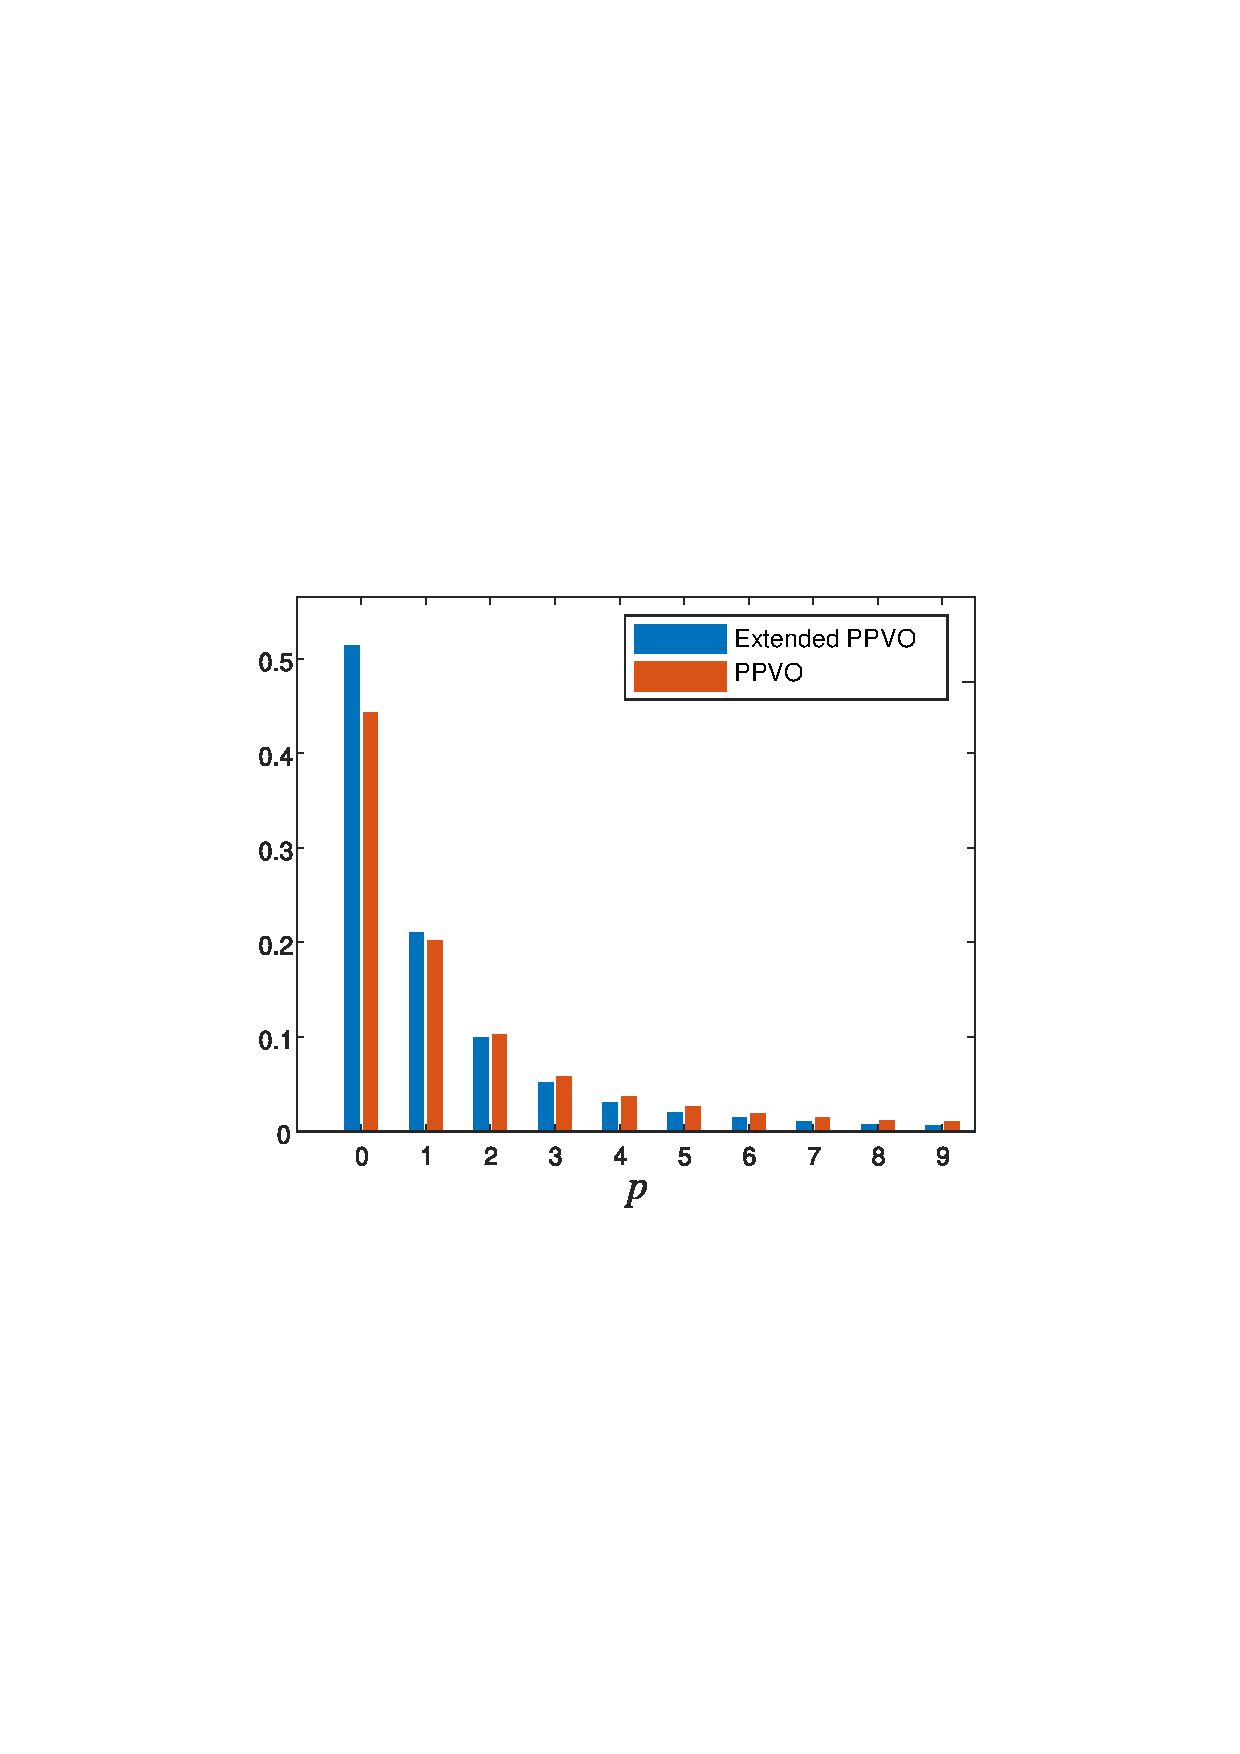
\includegraphics[width=1\textwidth]{figures/Comparison/airplane.pdf}
    \end{minipage}
}
\subfigure[Barbara]{
    \begin{minipage}[t]{0.225\linewidth}
    \centering
    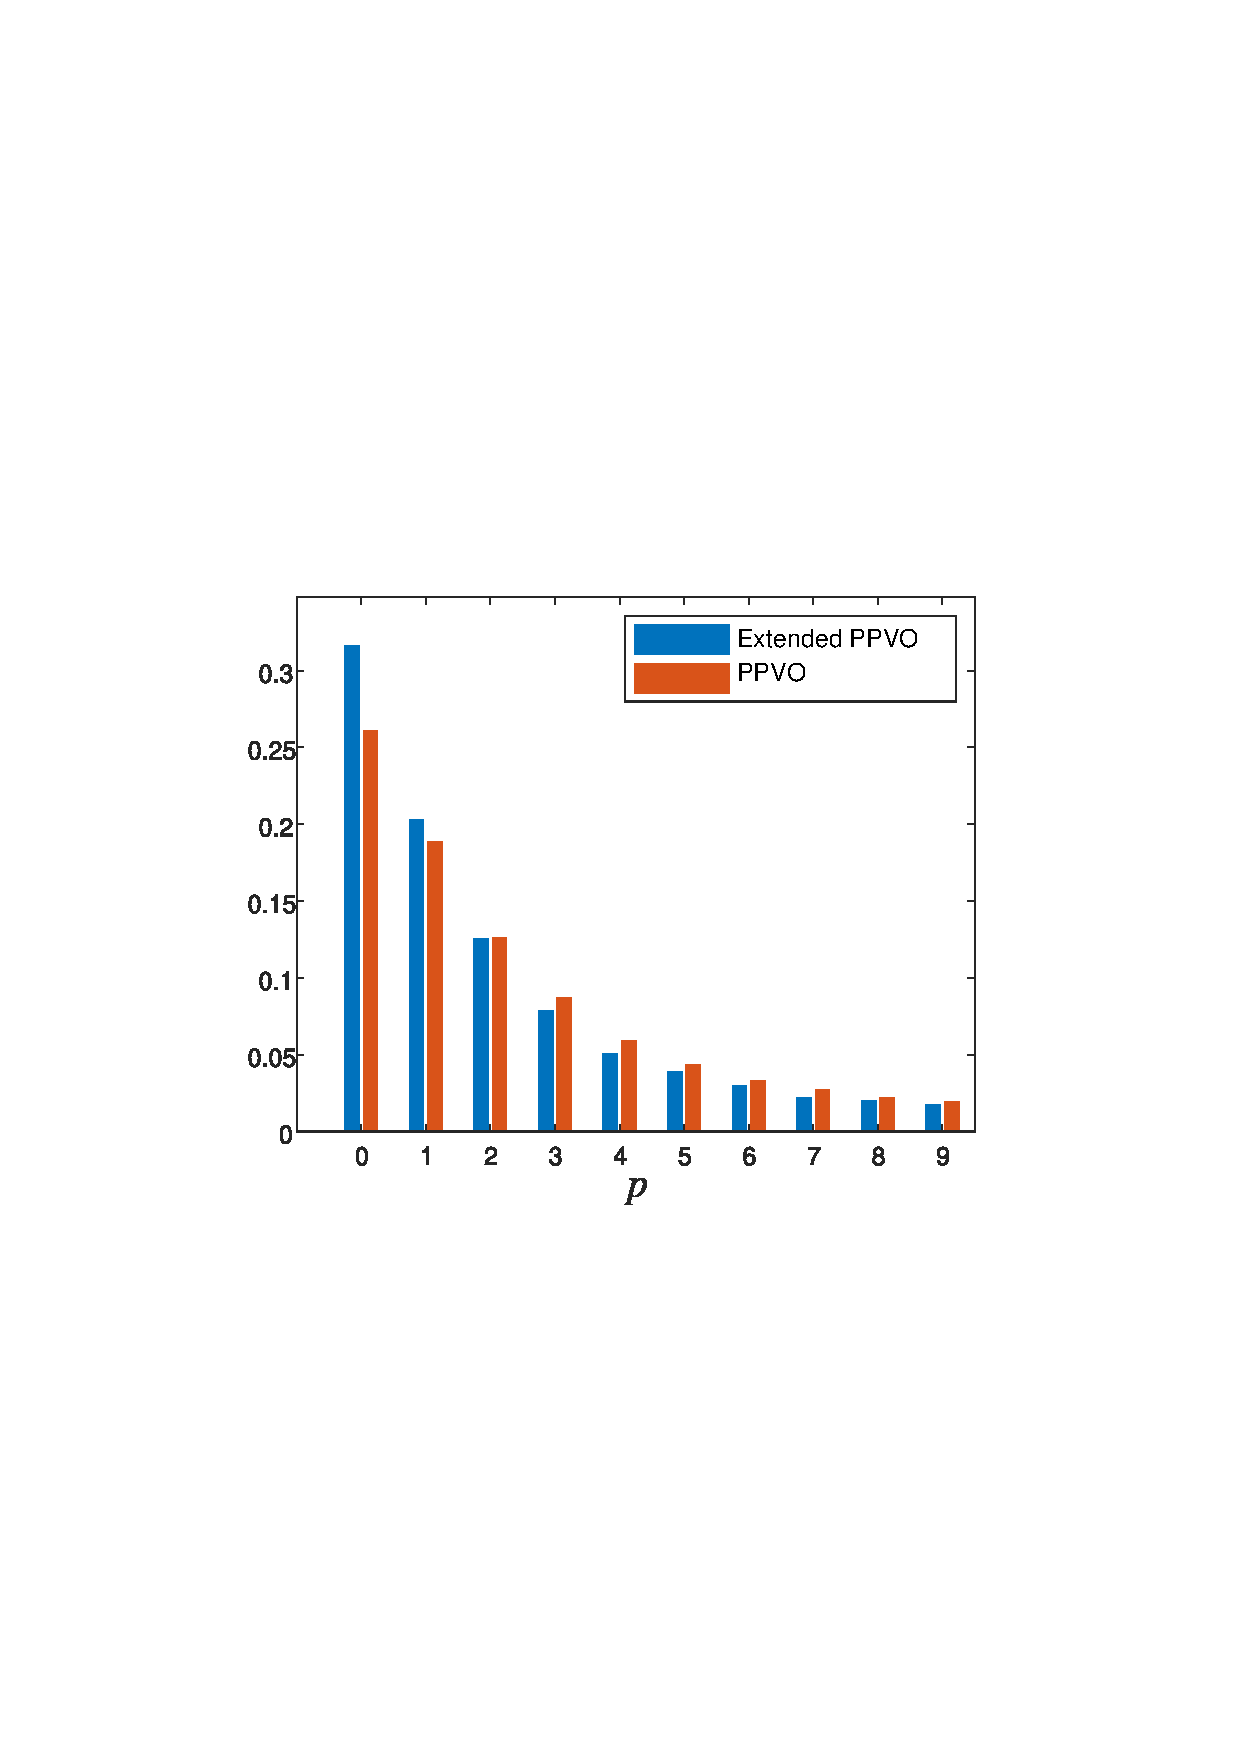
\includegraphics[width=1\textwidth]{figures/Comparison/barbara.pdf}
    \end{minipage}
}


\subfigure[Lake]{
    \begin{minipage}[t]{0.225\linewidth}
    \centering
    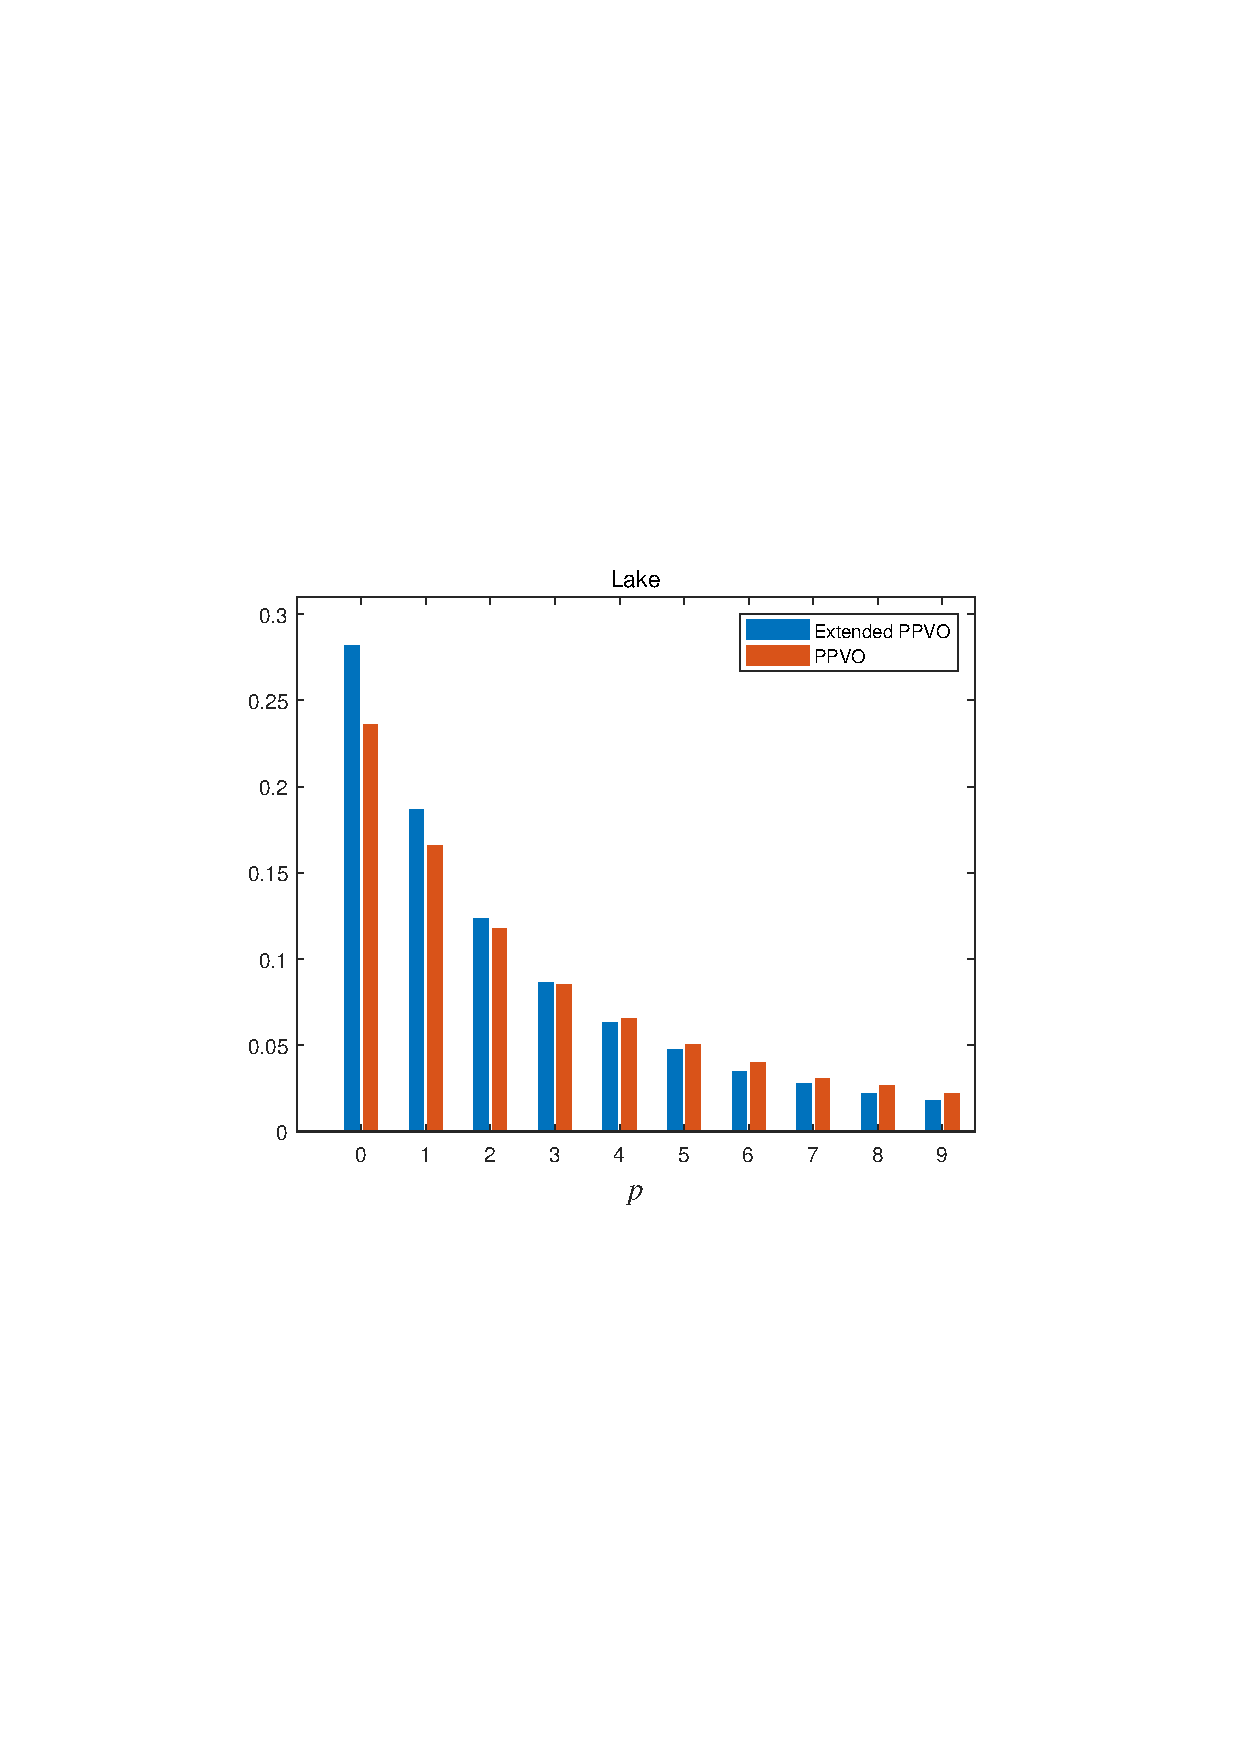
\includegraphics[width=1\textwidth]{figures/Comparison/lake.pdf}
    \end{minipage}
}
\subfigure[Peppers]{
    \begin{minipage}[t]{0.225\linewidth}
    \centering
    \includegraphics[width=1\textwidth]{figures/Comparison/peppers.pdf}
    \end{minipage}
}
\subfigure[Boat]{
    \begin{minipage}[t]{0.225\linewidth}
    \centering
    \includegraphics[width=1\textwidth]{figures/Comparison/boat.pdf}
    \end{minipage}
}
\subfigure[Eliane]{
    \begin{minipage}[t]{0.225\linewidth}
    \centering
    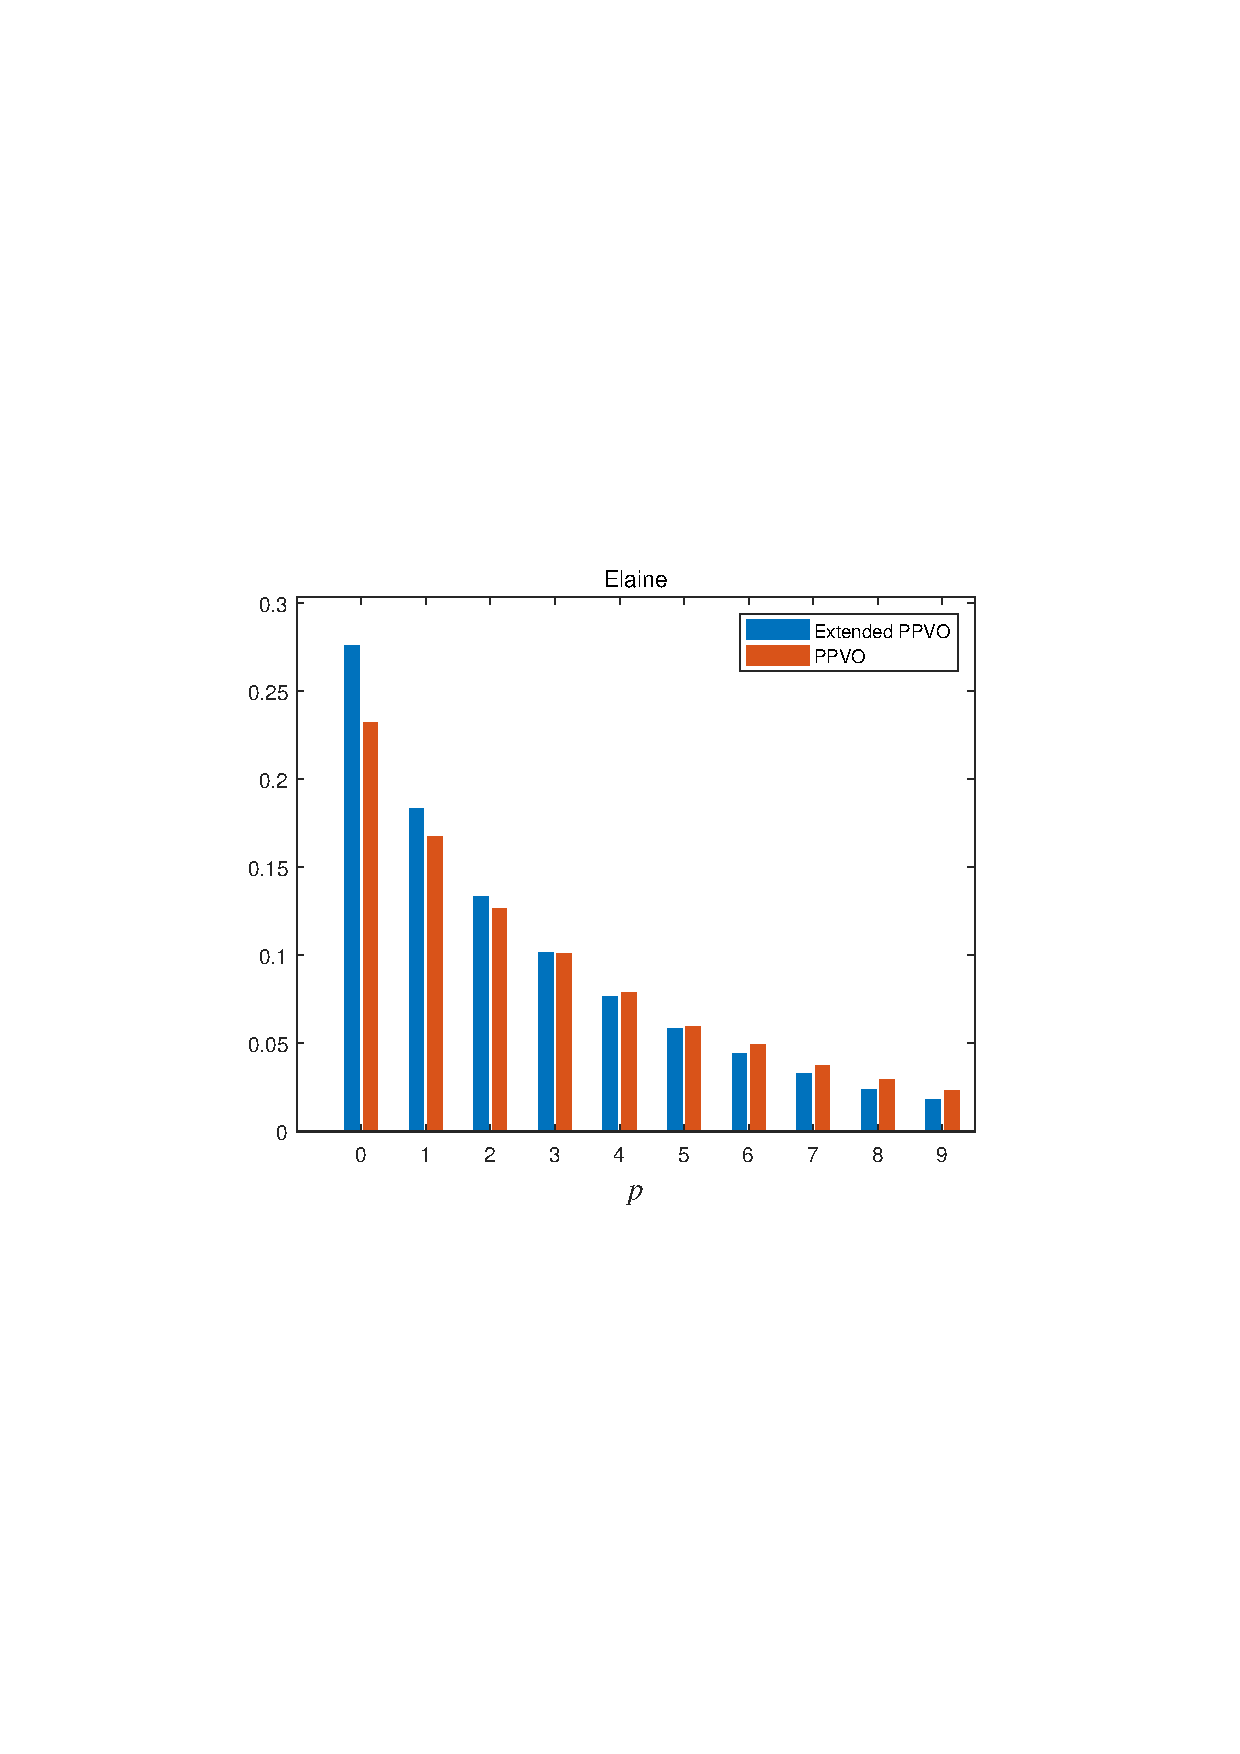
\includegraphics[width=1\textwidth]{figures/Comparison/elaine.pdf}
    \end{minipage}
}
\centering
\caption{Comparison of normalized prediction-errors $p$ of extended PPVO by (\ref{eq:EPPVOPE}) in blue and PPVO by (\ref{eq:PPVOPE}) in orange.}
\label{Fig.ComparisonEPPVO}
\end{figure*}


% embedding procedure
Next, 

% for reversibility(extraction procedure shown here?)

\subsection{Multi-size based Embedding Method for MHM}\label{sec:3.2}

%----------------------------------------------------------------------------------------
\section{Experimental Results}\label{sec:4}

%----------------------------------------------------------------------------------------
\section{Conclusion}\label{sec:5}

%----------------------------------------------------------------------------------------
\section*{Acknowledgement}


\bibliographystyle{elsarticle-num}

\bibliography{Cited}


\end{document}
